\documentclass[11pt]{article}
\usepackage{graphicx}
\usepackage {color}
\usepackage{pdfpages}
\usepackage{float}
\usepackage{changebar}
\usepackage{enumitem,amssymb}
\renewcommand{\familydefault}{\sfdefault}
\usepackage[margin=1.2in]{geometry}
\usepackage{graphicx}
\usepackage{wrapfig}
\usepackage[super]{cite}
\usepackage{subcaption}
\usepackage[table]{xcolor}
\usepackage{amsmath}
\usepackage[sort, numbers]{natbib}

%%%%%%%%%%%%Defining the margins %%%%%%%%%%%%%%%%%%%%%
\textheight 9.in
\textwidth 6.5in
\topmargin -.5in
\oddsidemargin 0in
\setlength{\parskip}{\smallskipamount}

%%%%%%%%%%%%%%Specific Commands %%%%%%%%%%%%%%%%%%
\newcommand{\eg}{{\em e.g.,}}
\newcommand{\ie}{{\em i.e.,}}
\newcommand{\etc}{{\em etc.,}}
\newcommand{\etal}{{\em et al.}}
\newcommand{\degrees}{{$^{\circ}$}}
\newcommand{\fig}[1]{\textbf{Figure #1}}

%%%%%%%%%%%%%%%%%%%%%%%%%%%% Setting to control figure placement
% These determine the rules used to place floating objects like figures 
% They are only guides, but read the manual to see the effect of each.
\renewcommand{\topfraction}{.9}
\renewcommand{\bottomfraction}{.9}
\renewcommand{\textfraction}{.1}
\renewcommand{\familydefault}{\sfdefault} %setting the san serif font

%%%%%%%%%%%%%%%%%%%%%%%% Line spacing
% Use the following command for ``double'' spacing
%\setlength{\baselineskip}{1.2\baselineskip}
% and this one for an acceptable NIH spacing of 6lpi based on 11pt
%\setlength{\baselineskip}{.9\baselineskip}
% The baselineskip does not appear to work when we include a maketitle
% command in the main file.  Something there must set the line spacing
% If we use this next command, then things seem to work.
\renewcommand{\baselinestretch}{.9}

\setcounter{secnumdepth}{0} %make no numbers but have a table of contents


\begin{document}

\title{Lab 3, Calcium Transient Simulations}
\author{Jake Bergquist, u6010393}
\maketitle
\tableofcontents
\newpage

\section{Introduction}
\par{}
While a larger goal of projects such as the Pysiome Project and the Virtual Physiological Human project are to develop tissue, organ, and system models for human Physiology, smaller scale models such as ion channel models are a vital part of these projects.\cite{Fink2011} Mathematical and computational models of Ion channels provide a framework for highly controlled investigation of the properties of these channels as well as the combination of vast amounts of experimental data into a single comprehensive model.  The modeling of ion channels contributes greatly to an effort to integrate and interpret experimental data as well as provide a highly detailed way to perform precise and otherwise technically impractical hypothesis testing on such a fine scale.
\par{}
While there are a vast variety of modeling techniques that range from basic current modeling with Hodgkin and Huxley to computationally intensive atomic scale molecular models, more frequently single ion channels are modeled using a Markovian chain of states model.\cite{Fink2011}\cite{Kojima2018a}
A Markovian model is one in which the next state of the model only depends on the current state, irrespective of the previous states. In the case of ion channels, Markovian models are typically structured into different closed and open states with rate constants that determine the probability of transitioning from one state to another. Each of these different states define different properties about the ion channel in the simulation, such as its permeability to ions, thus the effect on the conductance of those ions.\cite{Fink2011} In the most simple case of a two state Markovian ion channel model there is an open state and a closed state. At any given time the model may transition from closed to open or open to closed based on two rate constants, an open to closed rate, and a closed to open rate. If the closed to open rate constant were higher, this would describe a channel has a higher probability of being in the open state as opposed to the closed state. By increasing the number of states these models can be used to describe more complex behaviors such as channels with inactive states or drug/ligand binding that modulate activity. Each of these different state transitions have add rate coefficients describing the transitions between those states and other states, and thus a complex network can be built up.
\par{}
Each of the parameters that comprise the rate coefficients must be determined. Typically the values used come from direct experimental data from the channels of interest. This data includes structural information gained from crystallography, imaging data, genomic analysis, and perhaps most frequently from patch clamp electrical recordings. 

\section{Methods}
\par{}
All simulations during this lab were run using the JSim software and the Ten Tusscher Cell ML model described in \cite{TenTusscher2003}. Parameters were left at default unless otherwise stated, and figures were generated from screen capture from the JSim output. Any mathematical processing down outside of the JSim software was done using MATLAB, and the code used is appended at the end of this report in the appendix.

\subsection{1:Modeling of Repolarization}
The purpose of this section was to assess the effects of changes to the hERG potassium channel, particularly relating to the repolarization of the cell model. The simulation was run at default paprameters, then the again with the hERG conductances set to 200 \%, 50 \%, and 0 \% of the default conductance (0.0192, 0.048, 0 nanoseimens/picosecond
respectively). For each simulation the generated action potential was plotted  and captured using JSim, and the APD90 was calculated for each. The APD90 was defined as the point at which the model had repolarized 90\% to the resting value, thus it was calculated according to Equation \ref{eq:ap90} where Vb is baseline voltage, Vp is peak voltage of the action potential. The action potential duration was then calculated as the time it took from the onset of the action potential (time of maximum upstroke) till the time that the model repolarized back to the calculated AP90 voltage (time of APD90 repolarization - time of maximal upstroke). These APD90 times as well as the general action potential morphologies were compared for each of the hERG conductances.

\begin{equation} 
V(AP90) = Vb + 0.1*(Vb-Vp)
\label{eq:ap90}
\end{equation}


\subsection{2: Modeling of Calcium Transients}
\par{}
The purpose of this section was to investigate changes in calcium conductance and their effects on time to peak and calcium recovery. Fist the model was run at baseline with default parameters. Next the calcium conductance (gCal) was adjusted to 200\%, 50\%, and 0\% of the default value (0.35, 0.0875, 0
L/(faradsSeconds) respectively). The simulation was run again for each of these conductances and the membrane voltage and intracellular calcium concentrations were plotted. The time to peak was calculated in matlab by subtracting the time of the onset of the action potential (the first time point where the potential deviated from the rest value) from the time at which the action potential reached its peak. A time constant was found for the intracellular calcium recovery by curing curve fitting. Only the section of the curve after the peak was considered for exponential decay model.

\section{Results and Discussion}
\subsection{Potassium Conductance}
\par{}
In \ref{fig:original} we see the the JSim input and output for the default model. This model was used as a basis for all of the other work in this report. The values manipulated in this model were the the g\_Kr and g\_Cal values. All other values were left constant.

\begin{figure}[H]
	\centering
	\centering
	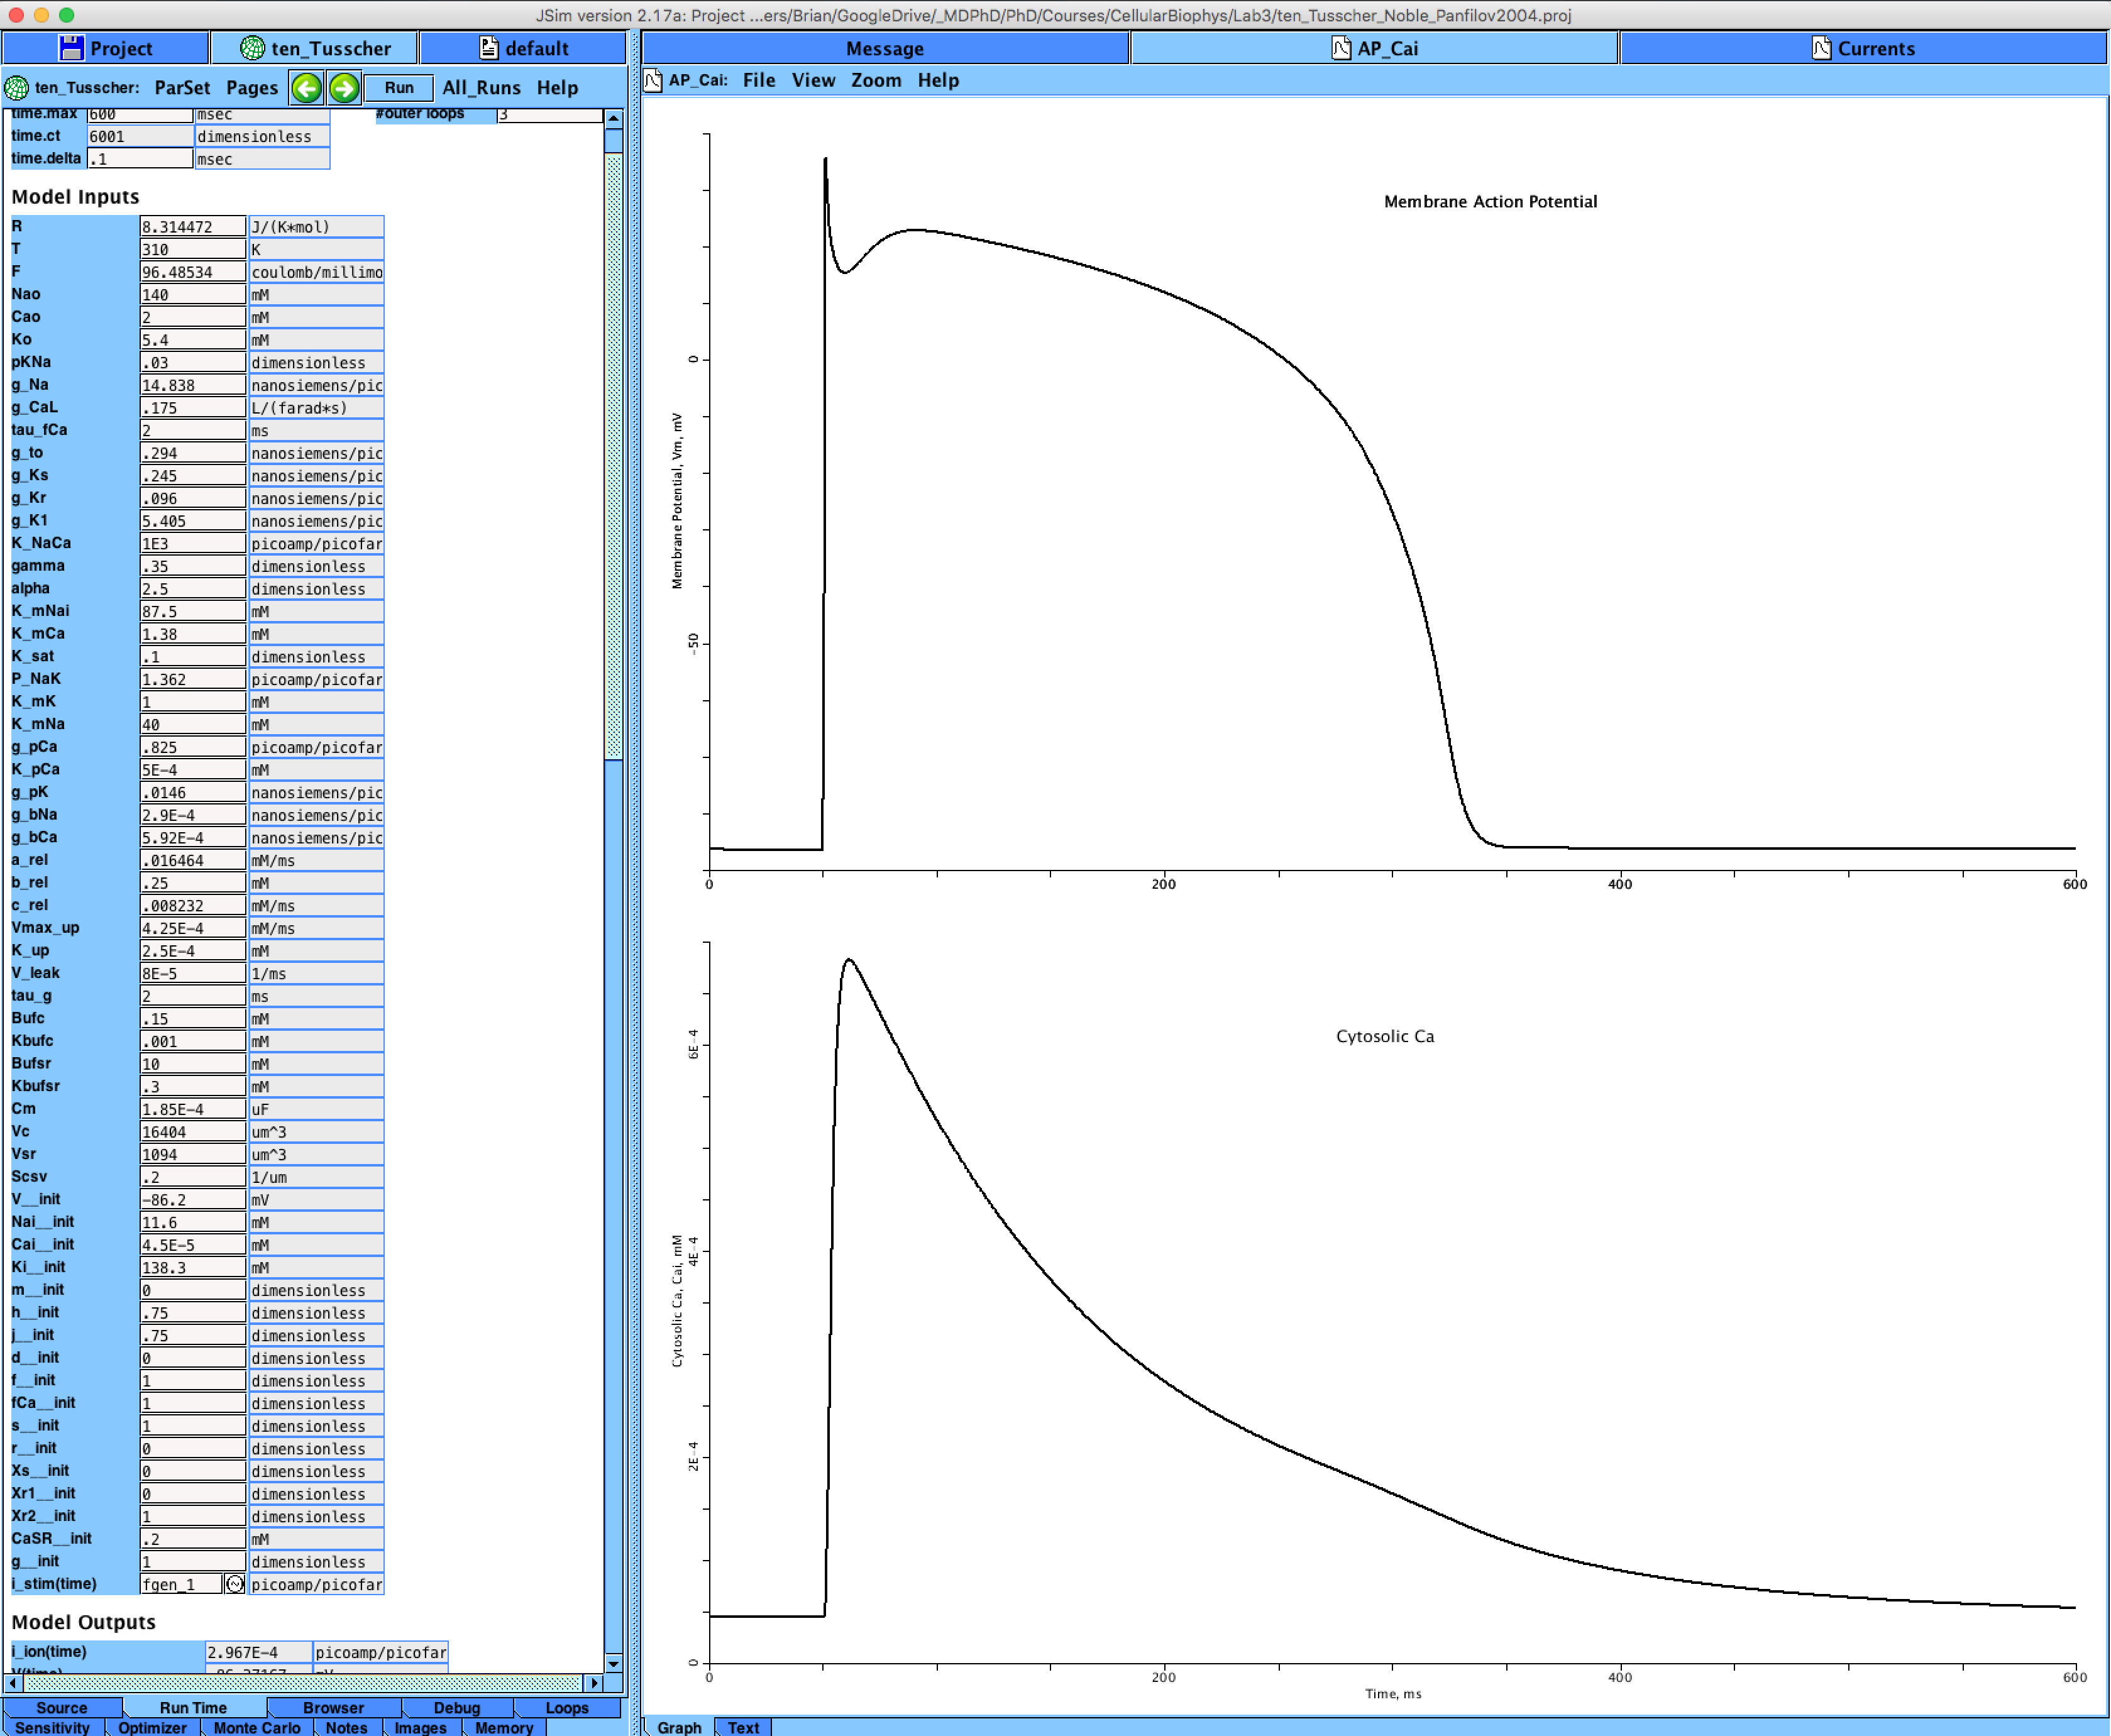
\includegraphics[width = .95\textwidth]{figs/original.png}
	
	\caption{Screen shot of JSim simulation inputs and outputs. The graphs show the simulated membrane potentials and intracellular Calcium transient. All parameters were left default for this run. }
	\label{fig:original}
\end{figure}
\par{}

In Figure \ref{fig:exp1} we see the result of altering the hERG potassium conductance (g\_Kr) on the membrane voltage. In particular we notice the change in the plateau and downslope of the action potential. Given the model, this makes sense. As hERG potassium conductance increases, the length of the action potential decreases. This is because hERG potassium is one of the main components driving repolarization of the membrane during an action potential. At lower hERG conductances, potassium cannot readily flow through the membrane and thus it cannot repolarize as quickly. At much higher hERG conductances potassium can easily flow out of the cell to cause rapid repolarization. This is seen in Figure \ref{fig:exp1} as each increase in the hERG conductance results in a decreased time to the initiation of repolarization.

\begin{figure}[H]
	\centering
	\begin{subfigure}{0.45\textwidth}
		\centering
		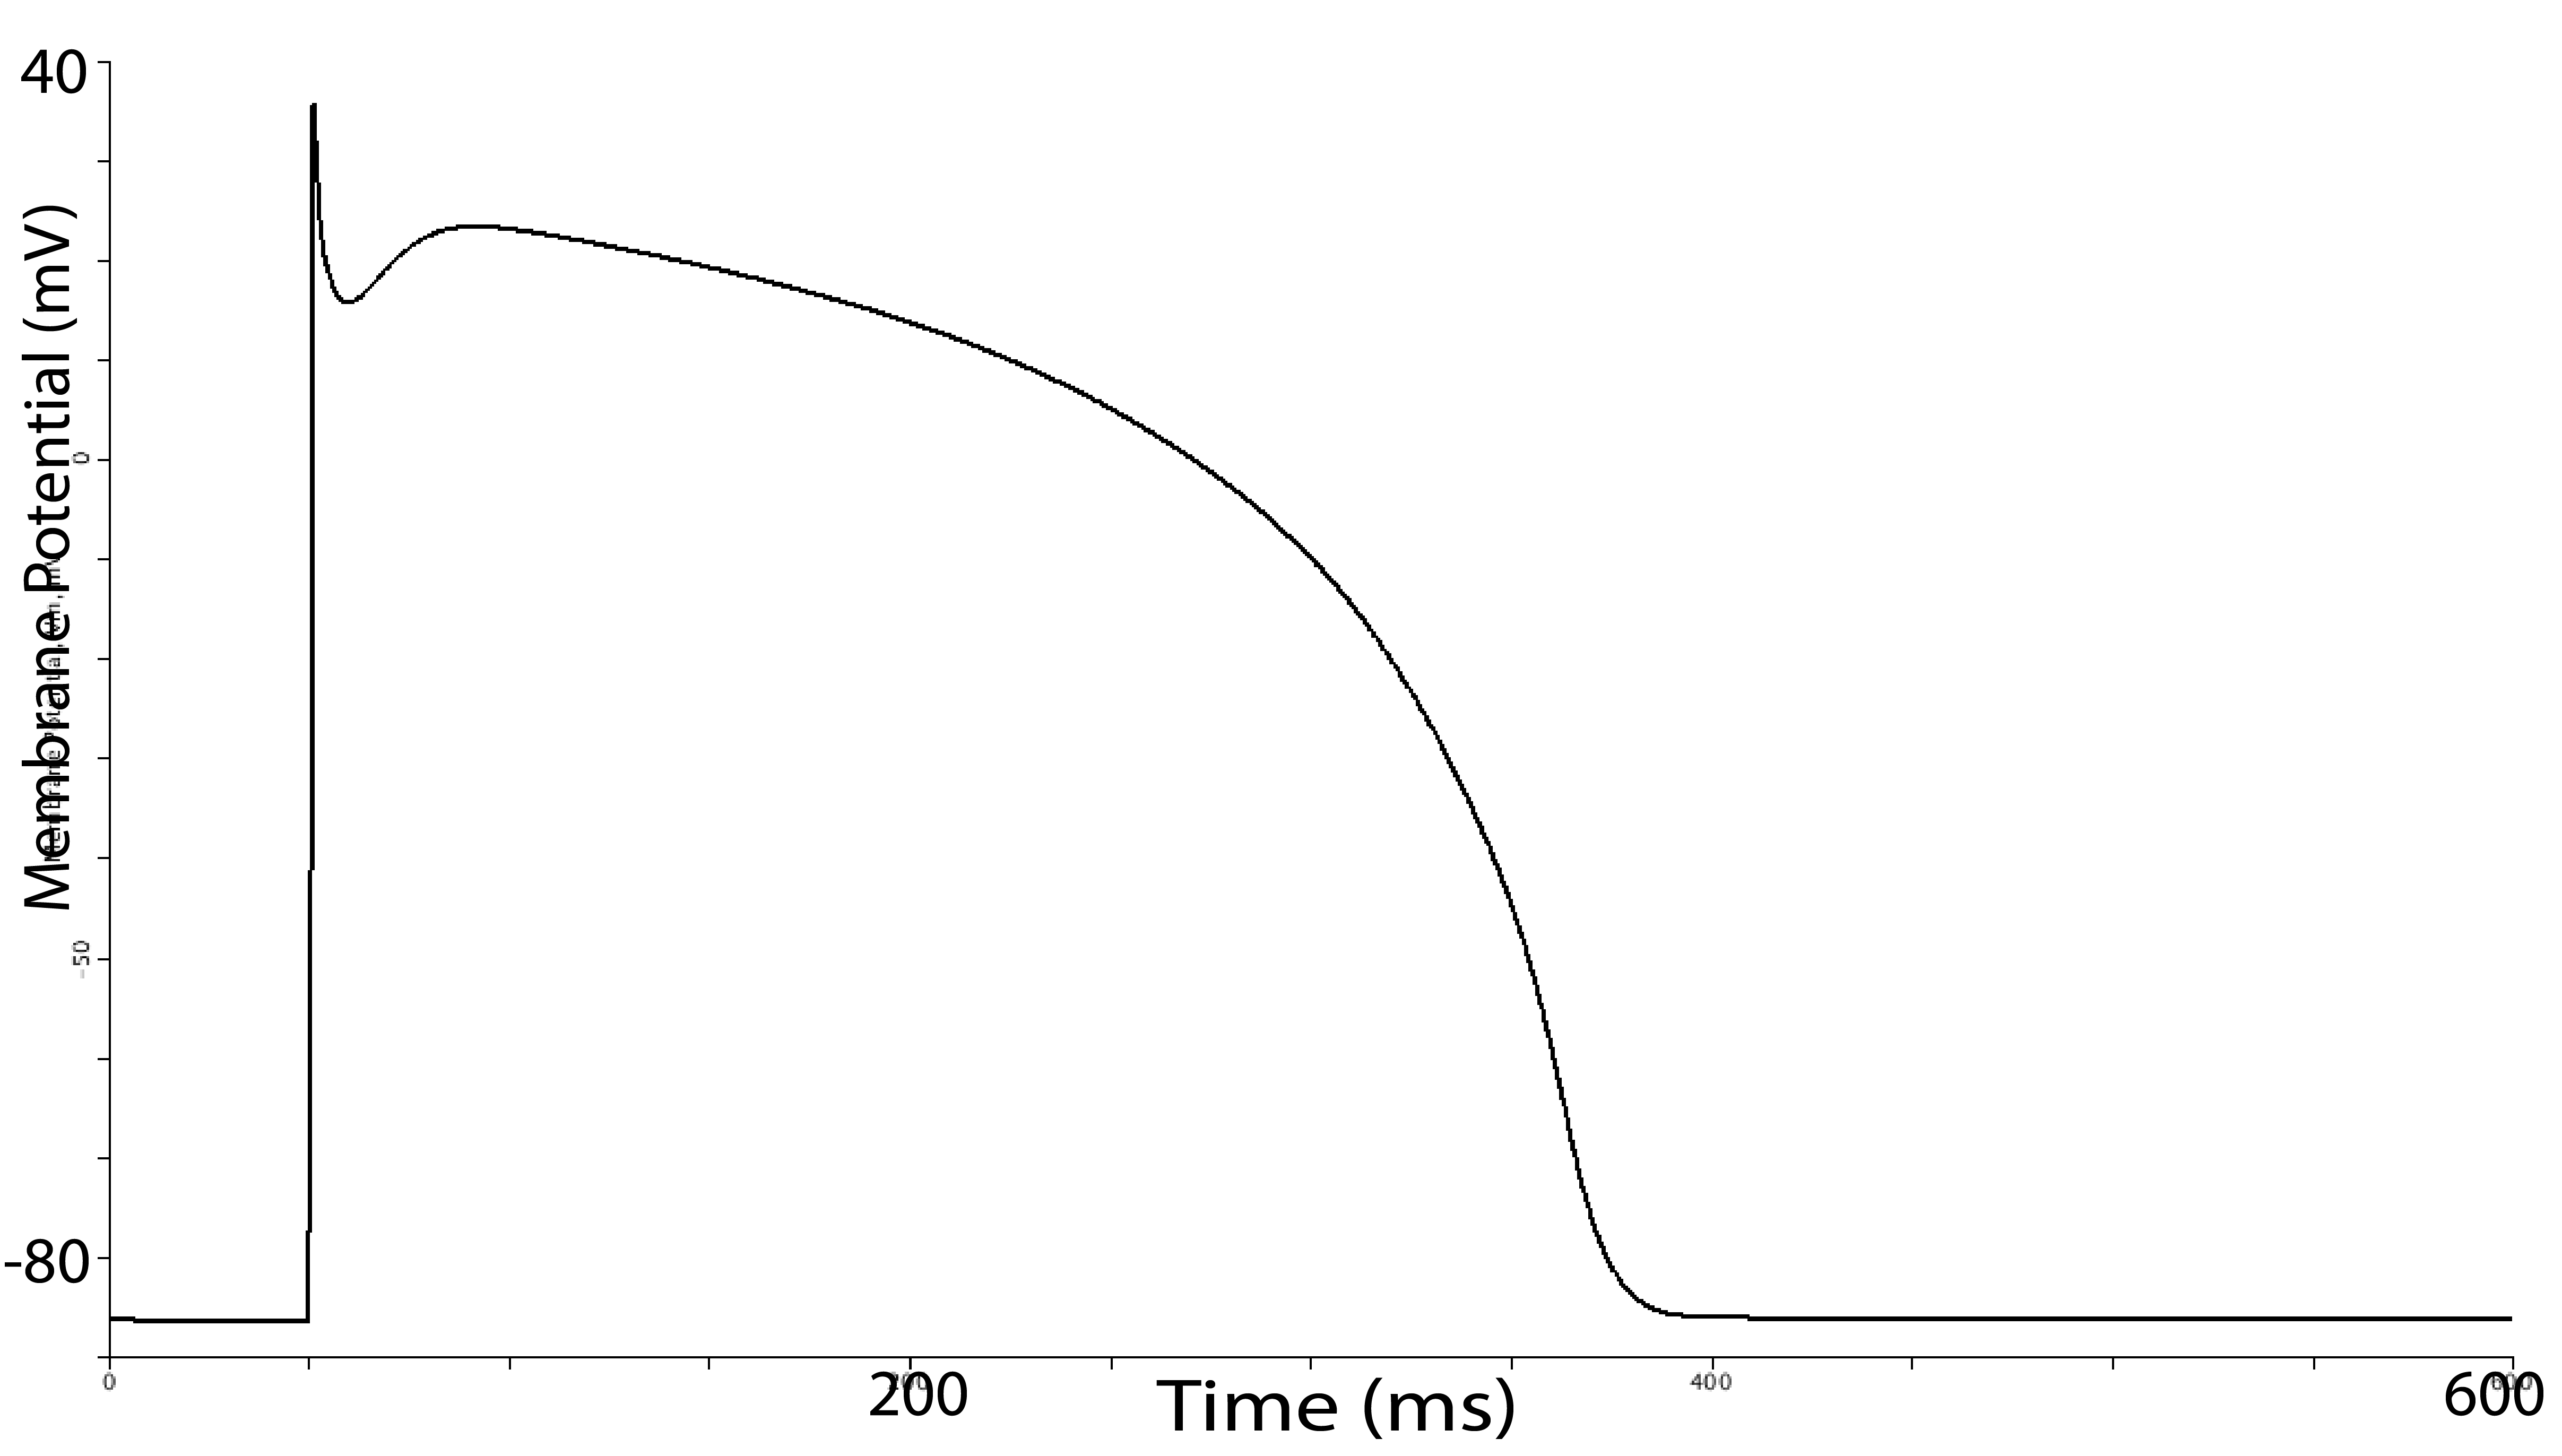
\includegraphics[width = \textwidth]{figs/0gkredit.png}
		\caption{}
		\label{exp1:a}
	\end{subfigure}
	\begin{subfigure}{0.45\textwidth}
		\centering
		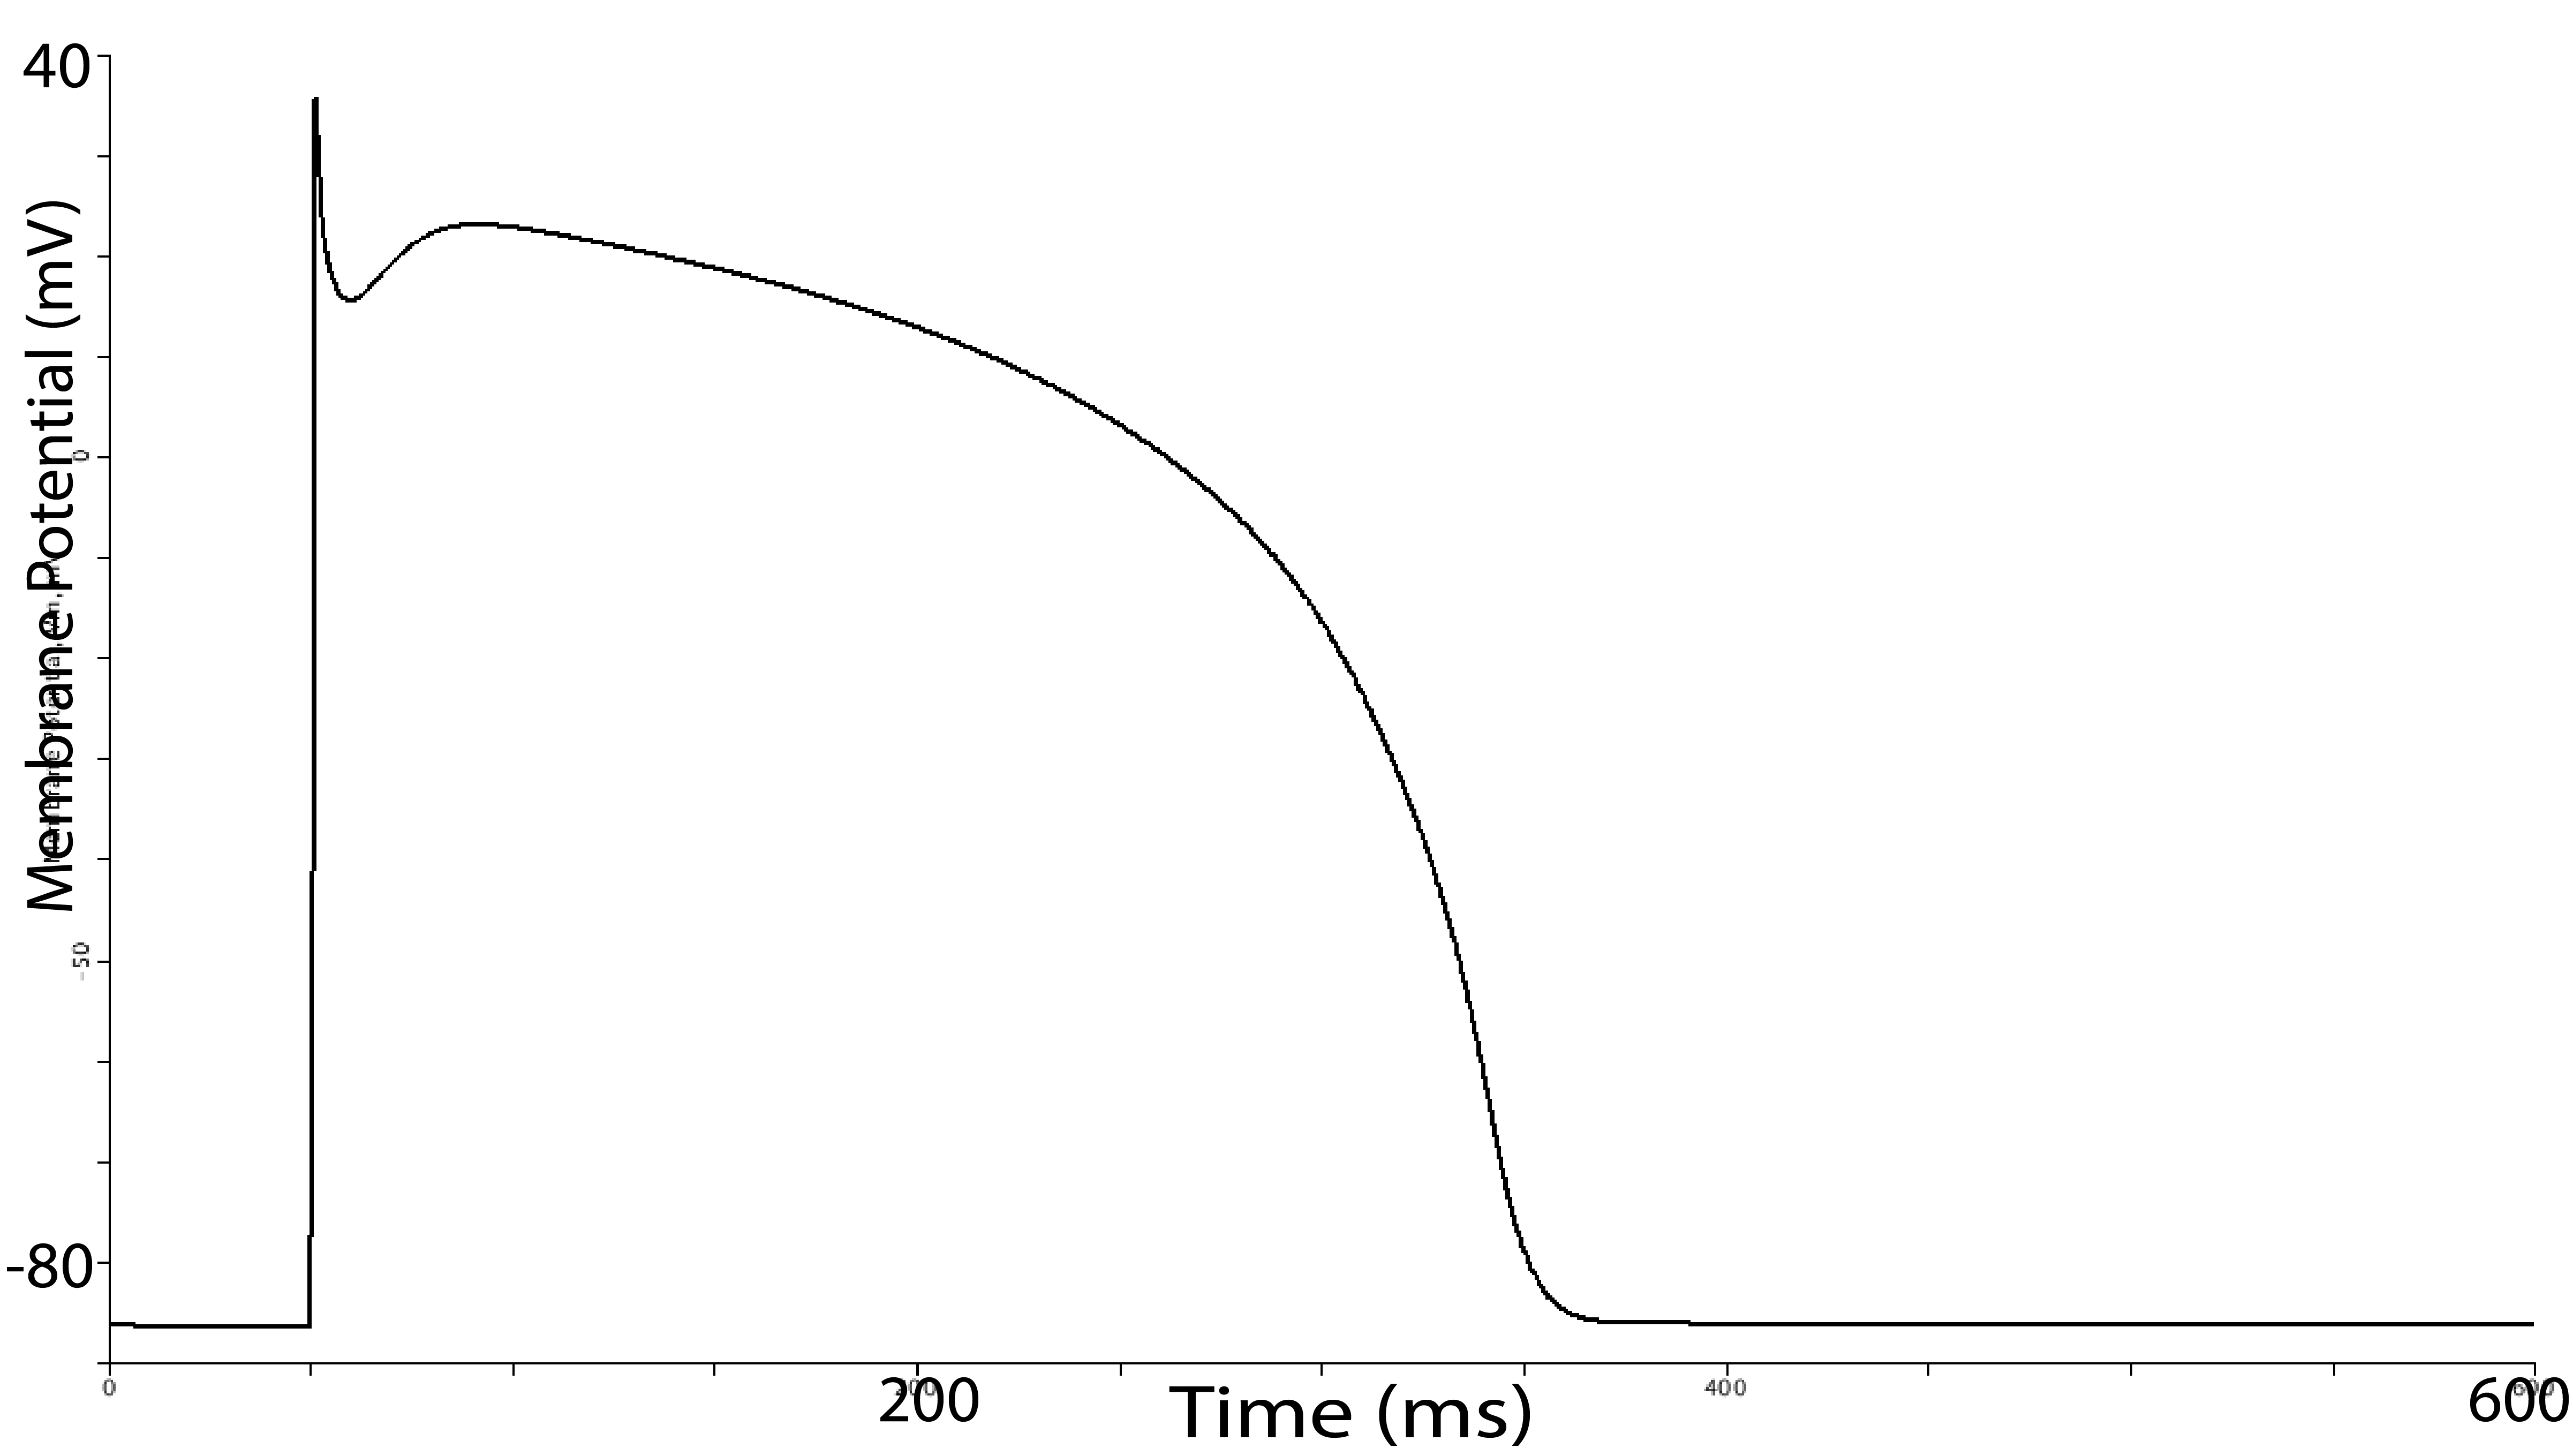
\includegraphics[width = \textwidth]{figs/50gkredit.png}
		\caption{}
		\label{exp1:b}
	\end{subfigure}
	\vskip\baselineskip
	\begin{subfigure}{0.45\textwidth}
		\centering
		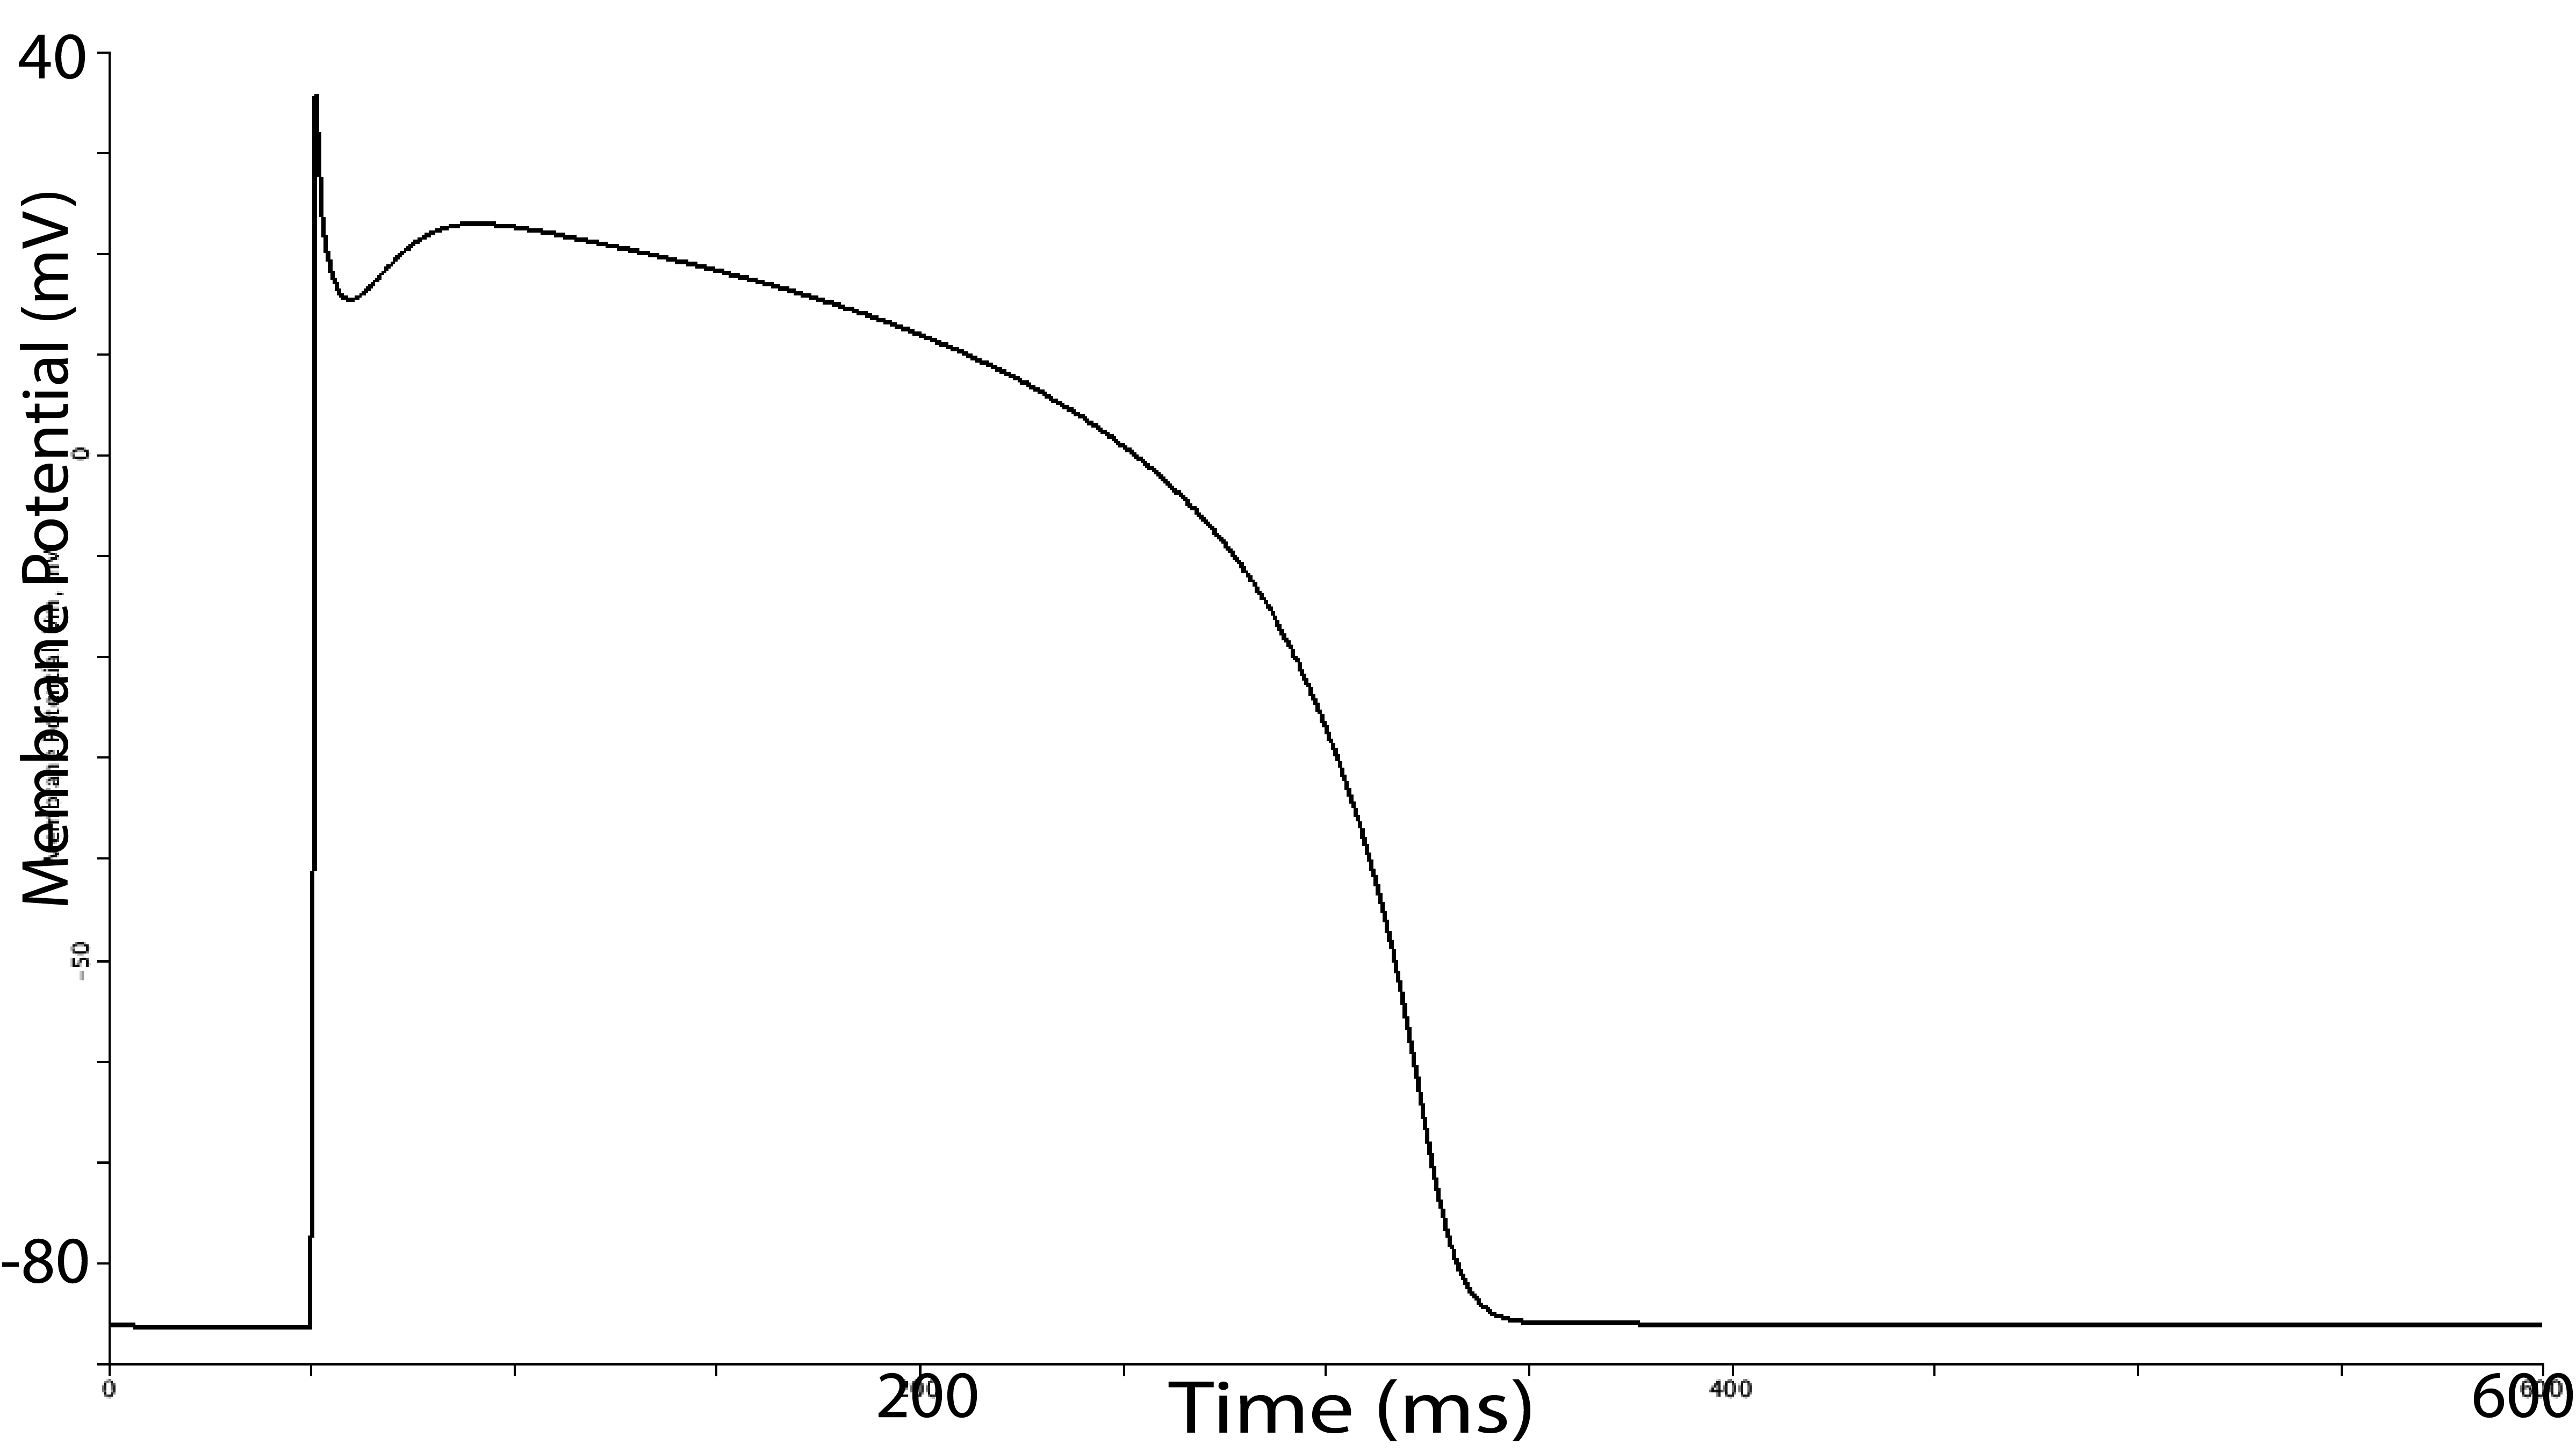
\includegraphics[width = \textwidth]{figs/originaleditK.png}
		\caption{}
		\label{exp1:c}
	\end{subfigure}
	\begin{subfigure}{0.45\textwidth}
		\centering
		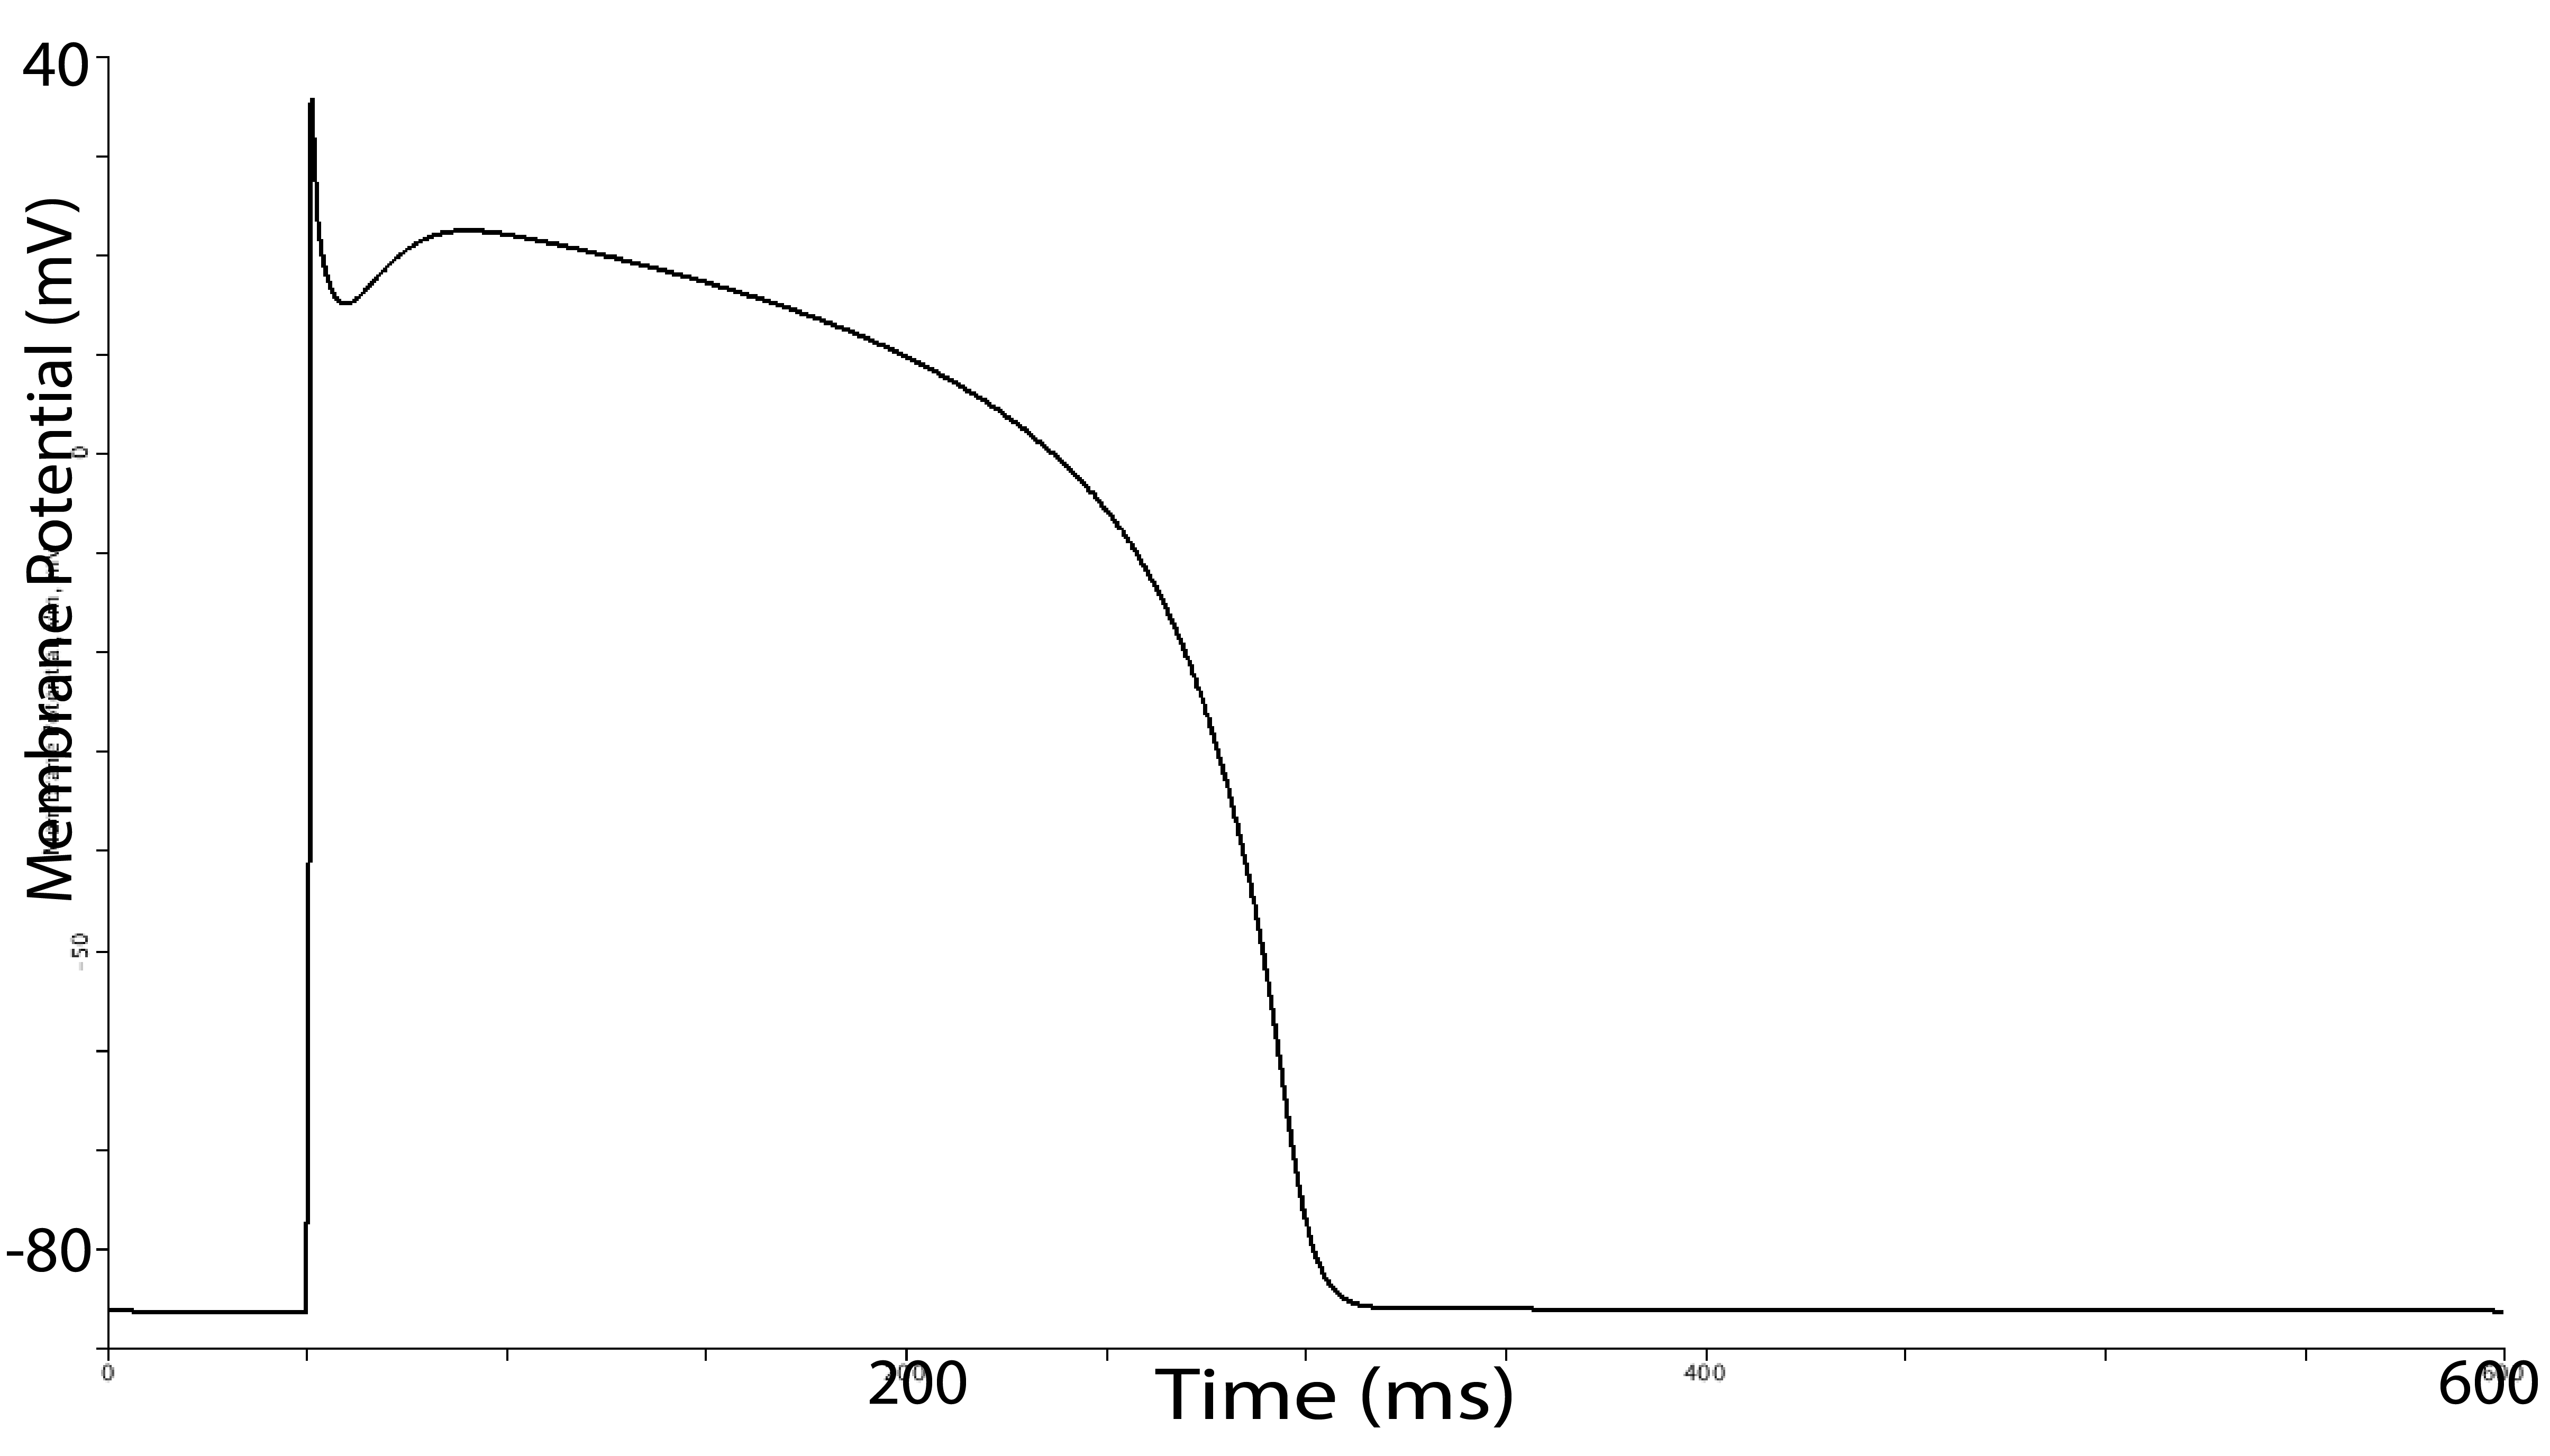
\includegraphics[width = \textwidth]{figs/200gkredit.png}
		\caption{}
		\label{exp1:d}
	\end{subfigure}
	\caption{Membrane potential at each conductance value for the hERG potassium channel after simulation. A: Conductance set to zero B. Conductance set to 50\% normal conductance, C: Conductance set to 100\% conductance, D: Conductance set to 200\% conductance. There is a marked decrease in action potential time with each increase in conductance. Units are in millivolts on the y axis and time (milliseconds) on the x axis}
	\label{fig:exp1}
\end{figure}
\par{}
To quantify this we calculated the APD90 time. This is the time it takes for the membrane to repolarize by 90\%, or reach a voltage that is 10\% of the peak voltage. The time of the beginning of the action potential (50 ms for our simulations) is then subtracted from these times to give us the APD90 time. These times are displayed in Table \ref{tab:potassium}. As can be seen, as conductance increases, ADP90 time decreases, as expected. Again this falls in line with our model as hERG contributes to repolarization. A lesser hERG conductance will result in a delayed reploarization, and therefore a higher APD90.

\rowcolors{2}{gray!25}{white}
\begin{table}[H]
	\centering
	\caption{Calculated APD90 times for each hERG channel conductance}
	\label{tab:potassium}
	\begin{tabular}{cc}
		\hline \hline
		hERG Conductance & APD90 (milliseconds)\\ 
		nanoseimens/picosecond &  \\
		\hline
		0\% Conductance & 318\\ 
		50\% Conductance &  297\\ 
		
		100\% Conductance &  278\\ 
		
		200\% Conductance&  249\\ 
		
		
		\hline 
		\hline
	\end{tabular} 
\end{table}
\par{}
These simulations can easily represent different physiological states for the hERG channel. In the case of lesser conductance, this could represent the effects of hERG blocker drugs or a mutated hERG channel that is less conductive to potassium. The increase hERG conductance tests can represent the effects of hERG activating drugs or activating mutations. In either case, the power of this simulation is that it allows for the exploration of these different situations. For example, suppose we have developed a drug that we want for treatment of a disease, but we learn through chemical analysis that it may affect the hERG conductance. We have three forms of the drug that change the hERG conductance by different amounts. By testing them in such a simulation as this we could investigate the effects of this drug on the cardiac action potential. Changes in the action potential such as those we see by varying the hERG conductance can have sever effects on cardiac health. Changes in repolarization time can lead to long or short QT syndrome, which are extensions or reductions iin the length of the qt segment of the ECG cause by longer or shorter repolarization/APD90 respectivly. Conditions such as these cna often cause lead to arrhythmia and even sudden cardiac death. 

\subsection{Calcium conductance}

\begin{figure}[H]
	\centering
	\begin{subfigure}{0.45\textwidth}
		\centering
		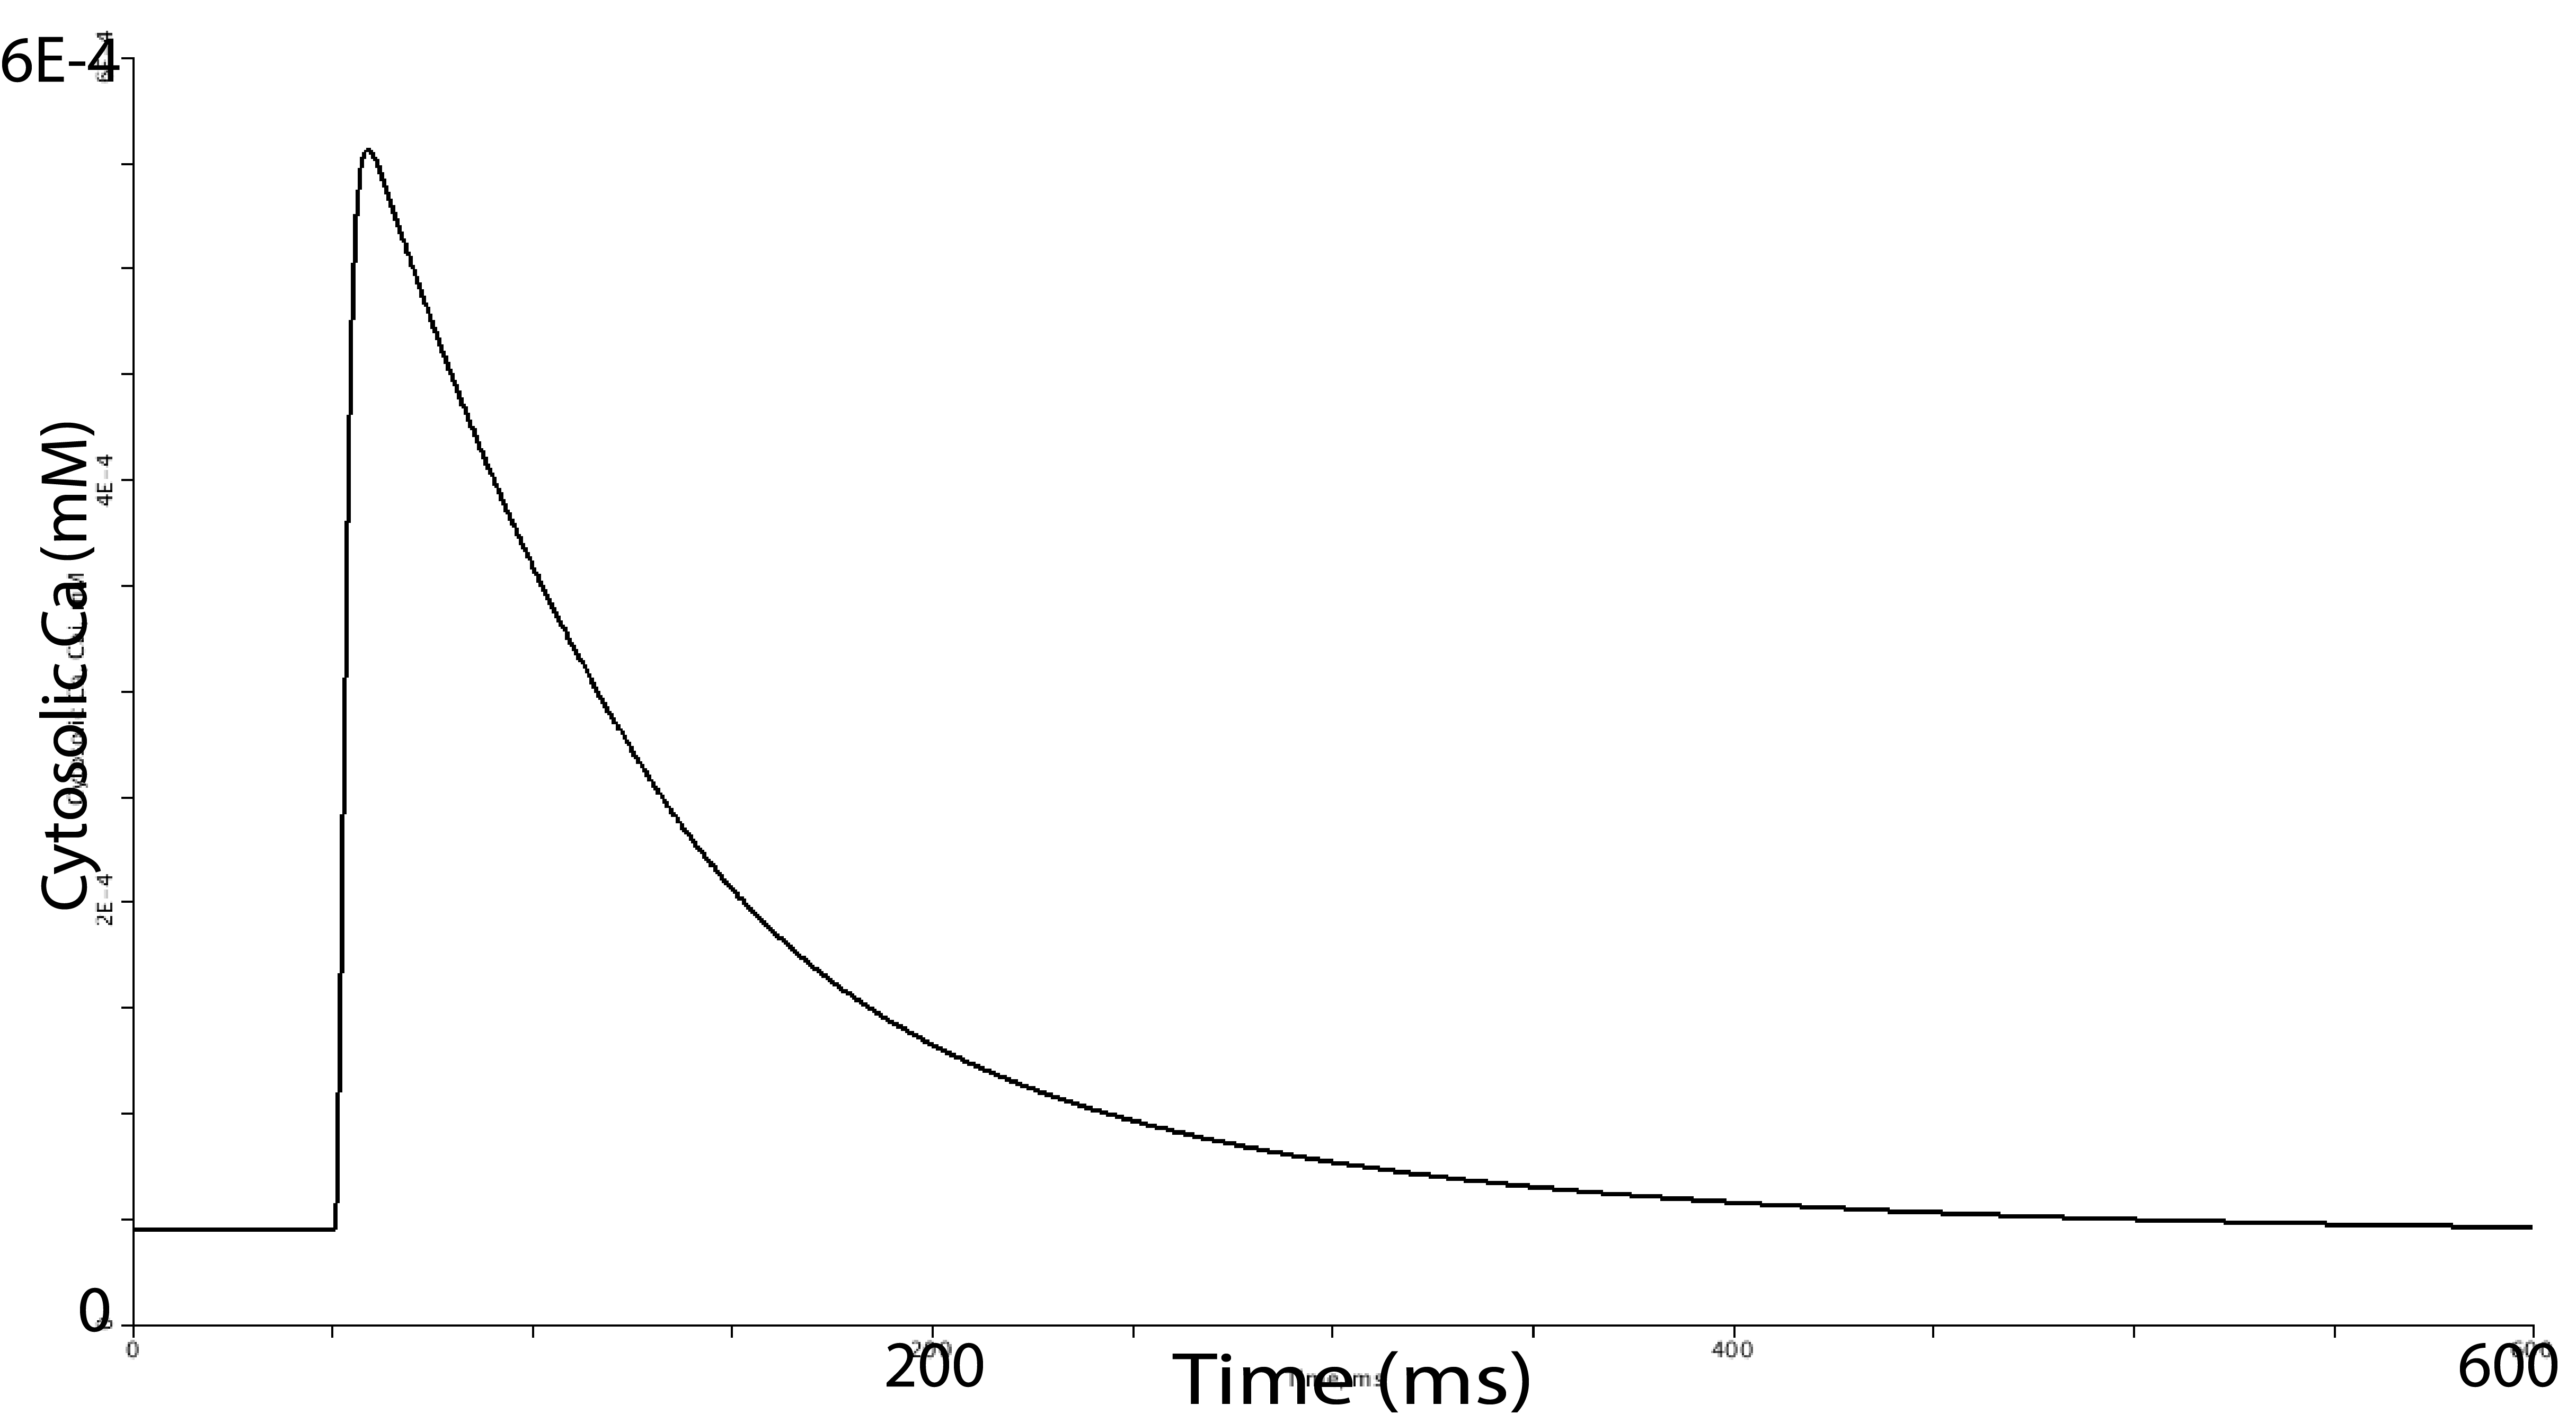
\includegraphics[width = \textwidth]{figs/0gcaledit.png}
		\caption{}
		\label{fig:left}
	\end{subfigure}
	\begin{subfigure}{0.45\textwidth}
		\centering
		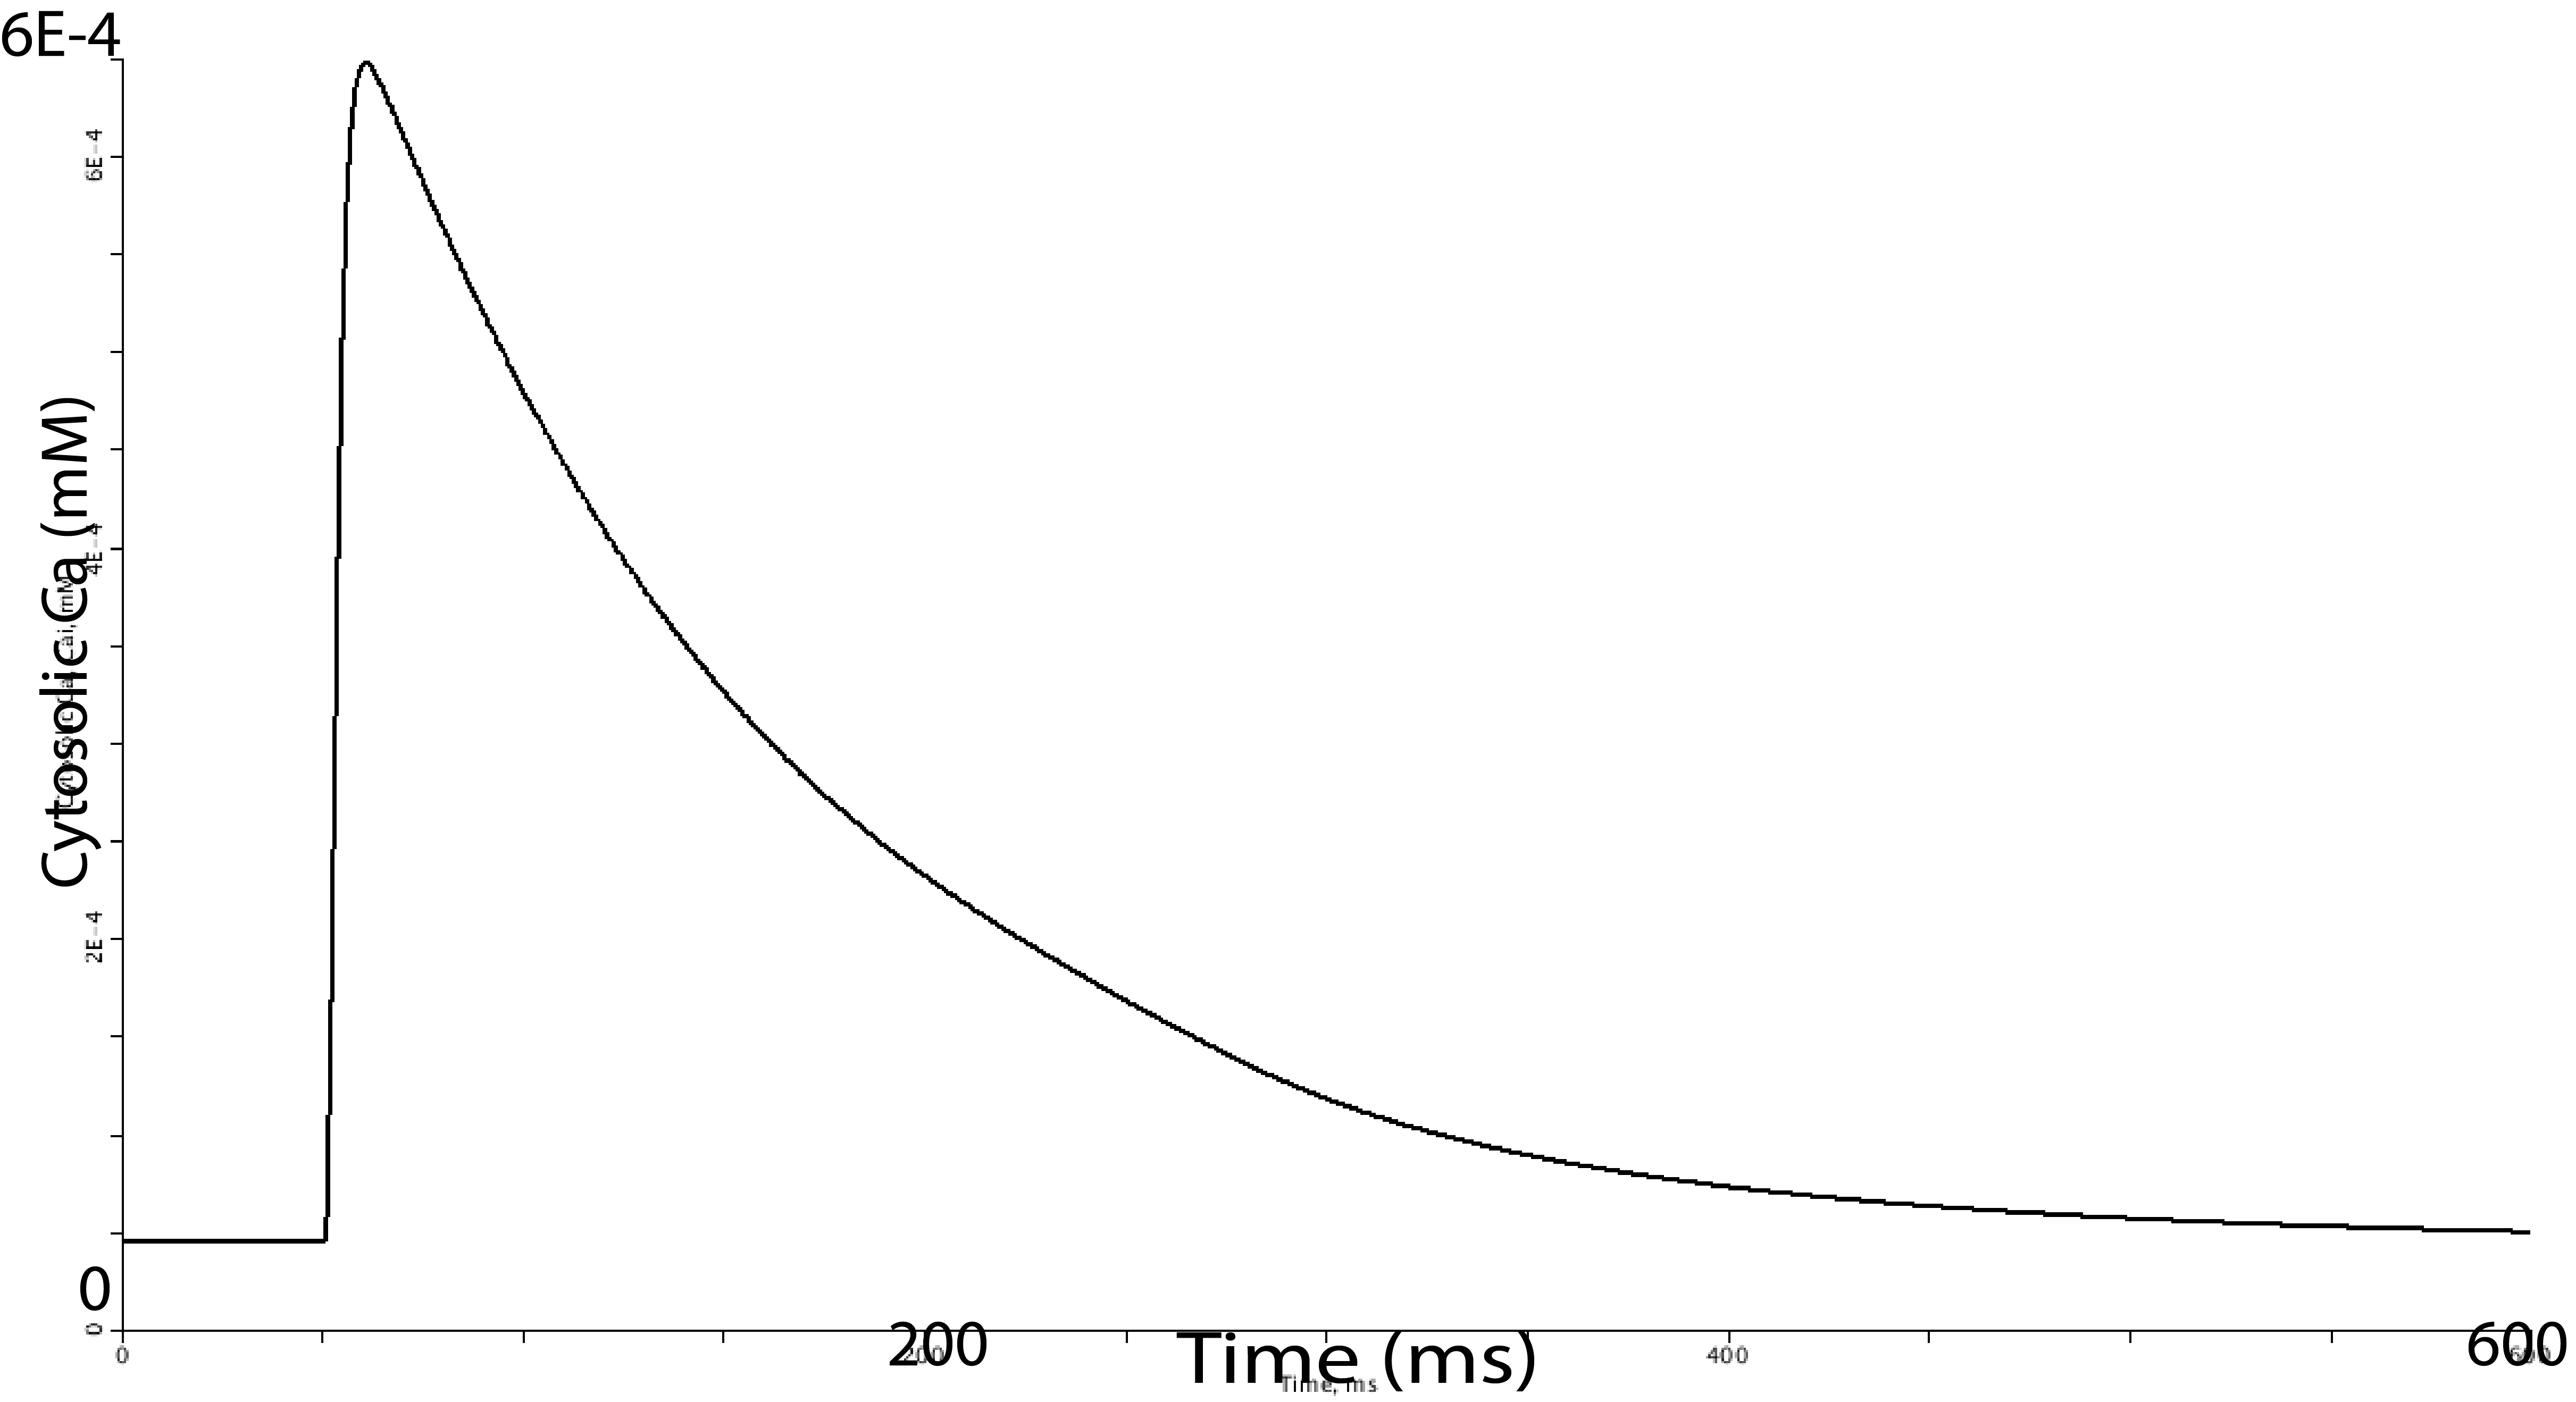
\includegraphics[width = \textwidth]{figs/50gcaledit.png}
		\caption{}
		\label{fig:right}
	\end{subfigure}
	\vskip\baselineskip
	\begin{subfigure}{0.45\textwidth}
		\centering
		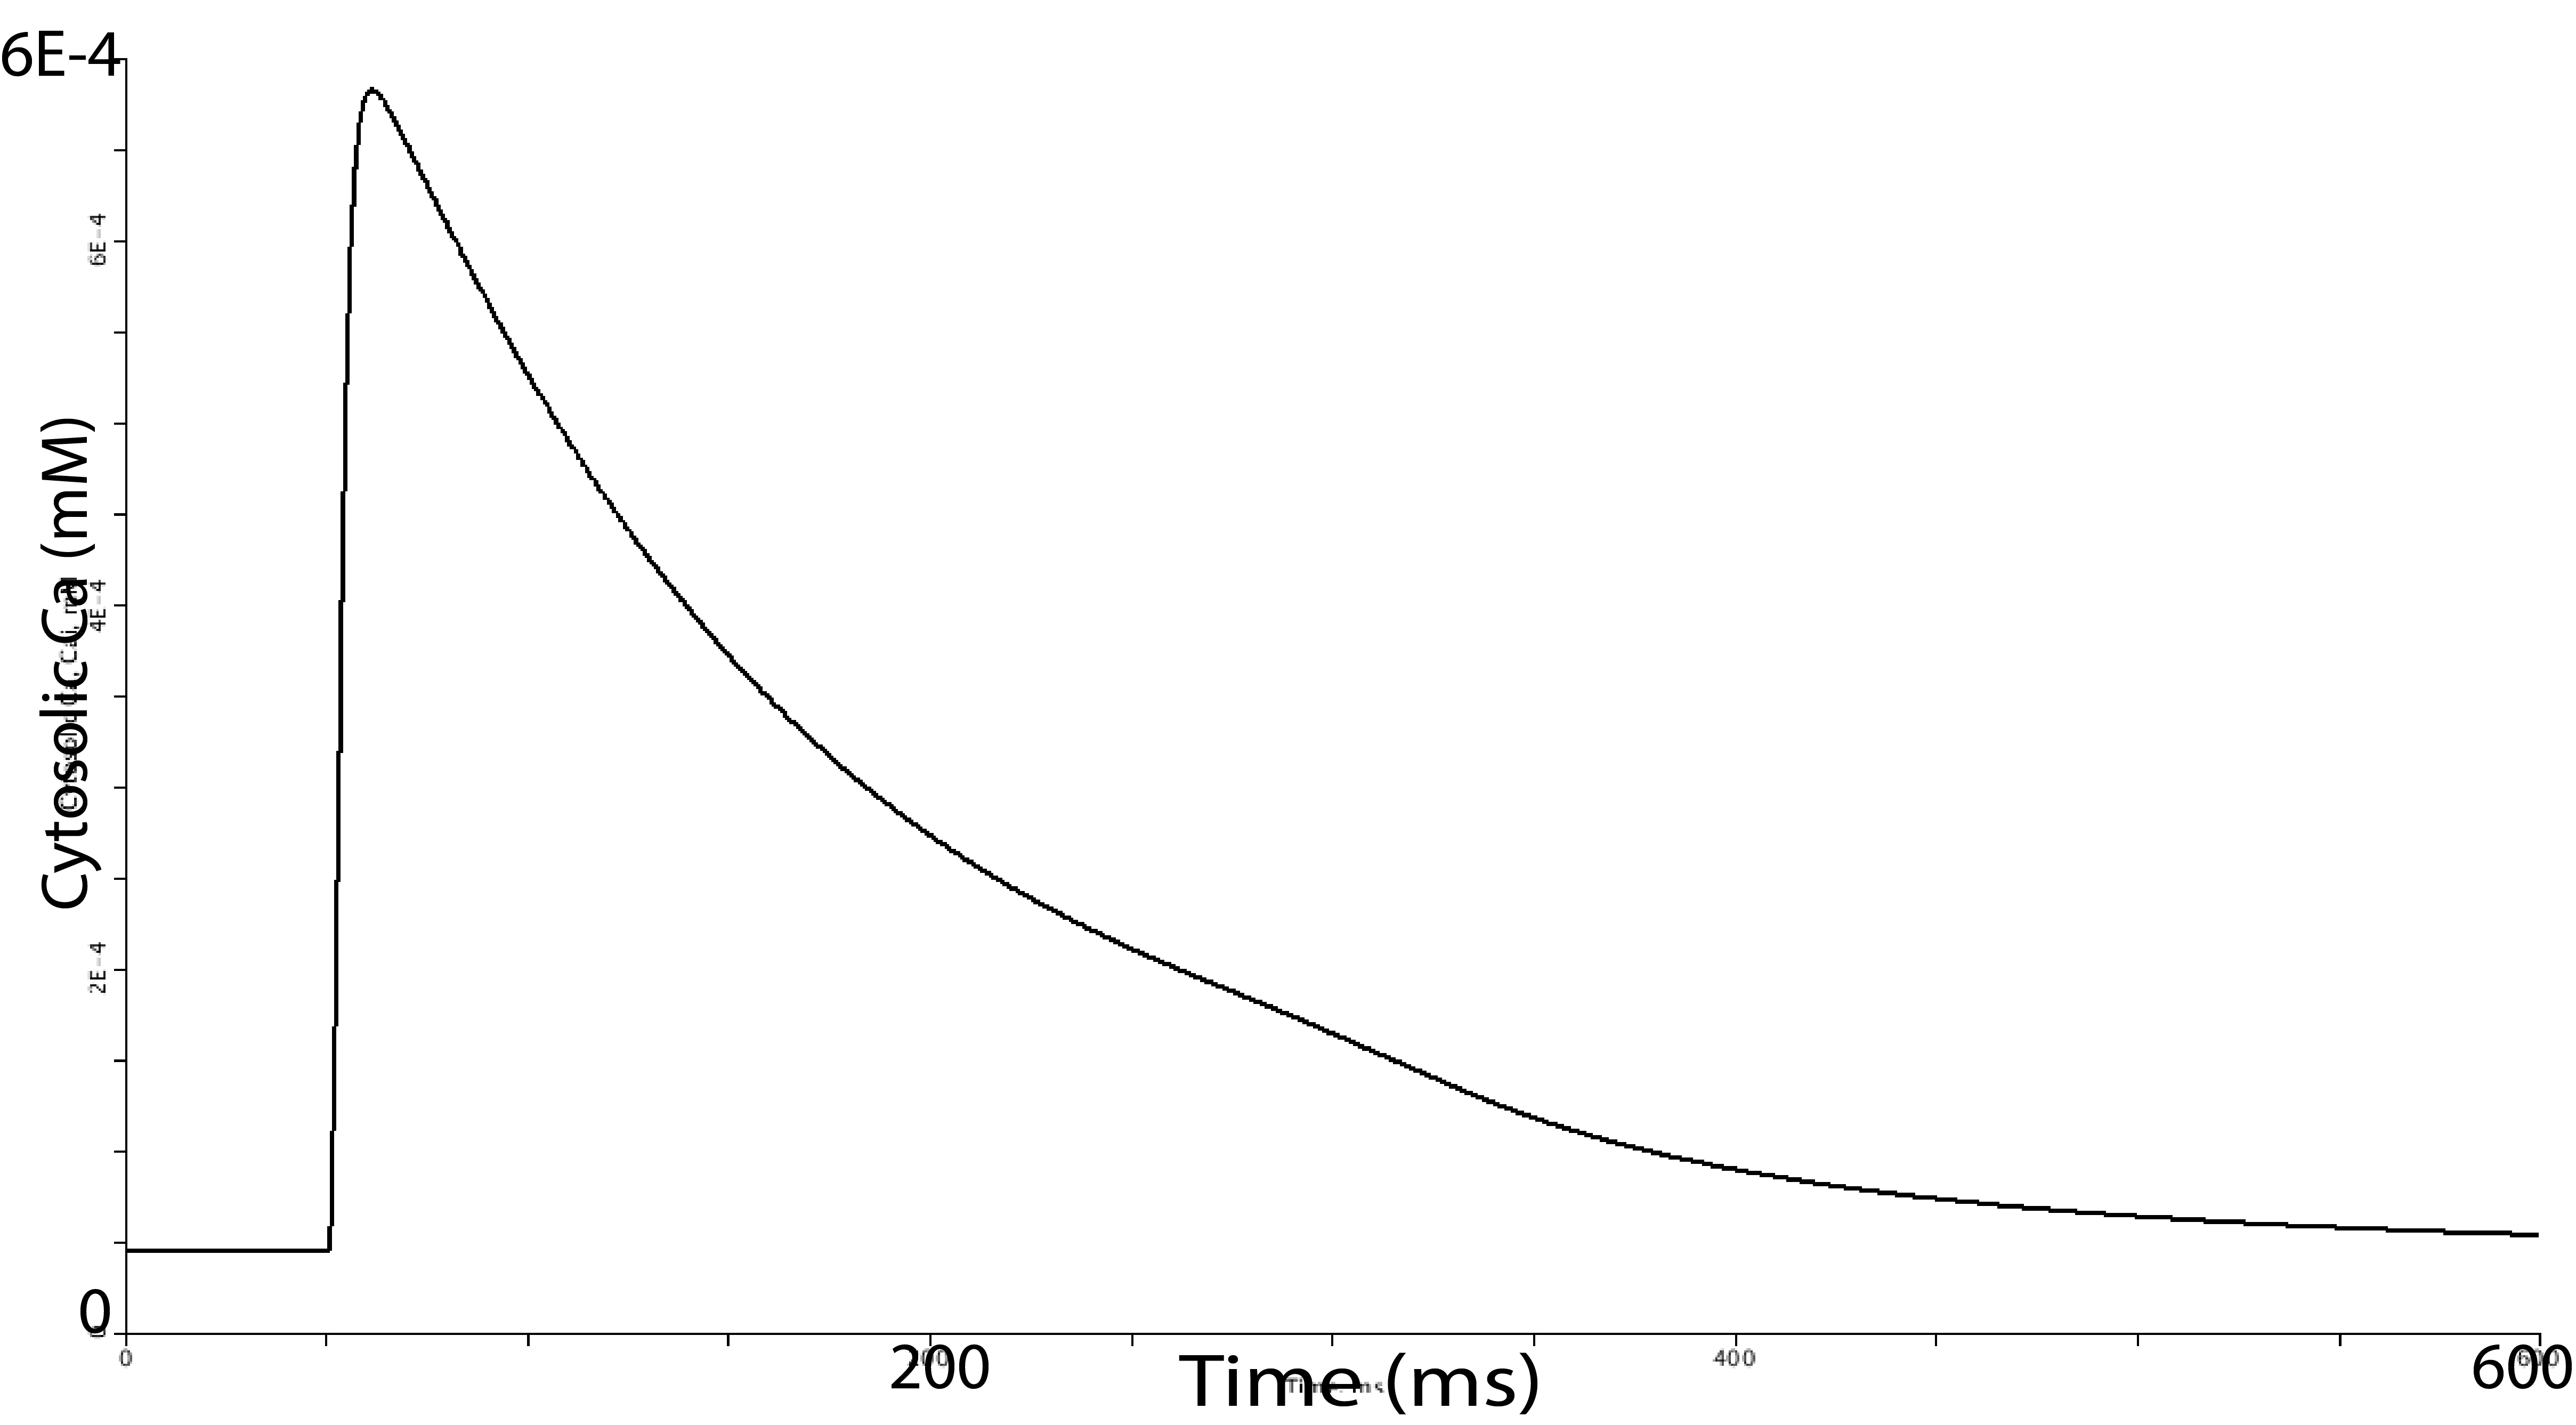
\includegraphics[width = \textwidth]{figs/originaleditCa.png}
		\caption{}
		\label{fig:left}
	\end{subfigure}
	\begin{subfigure}{0.45\textwidth}
		\centering
		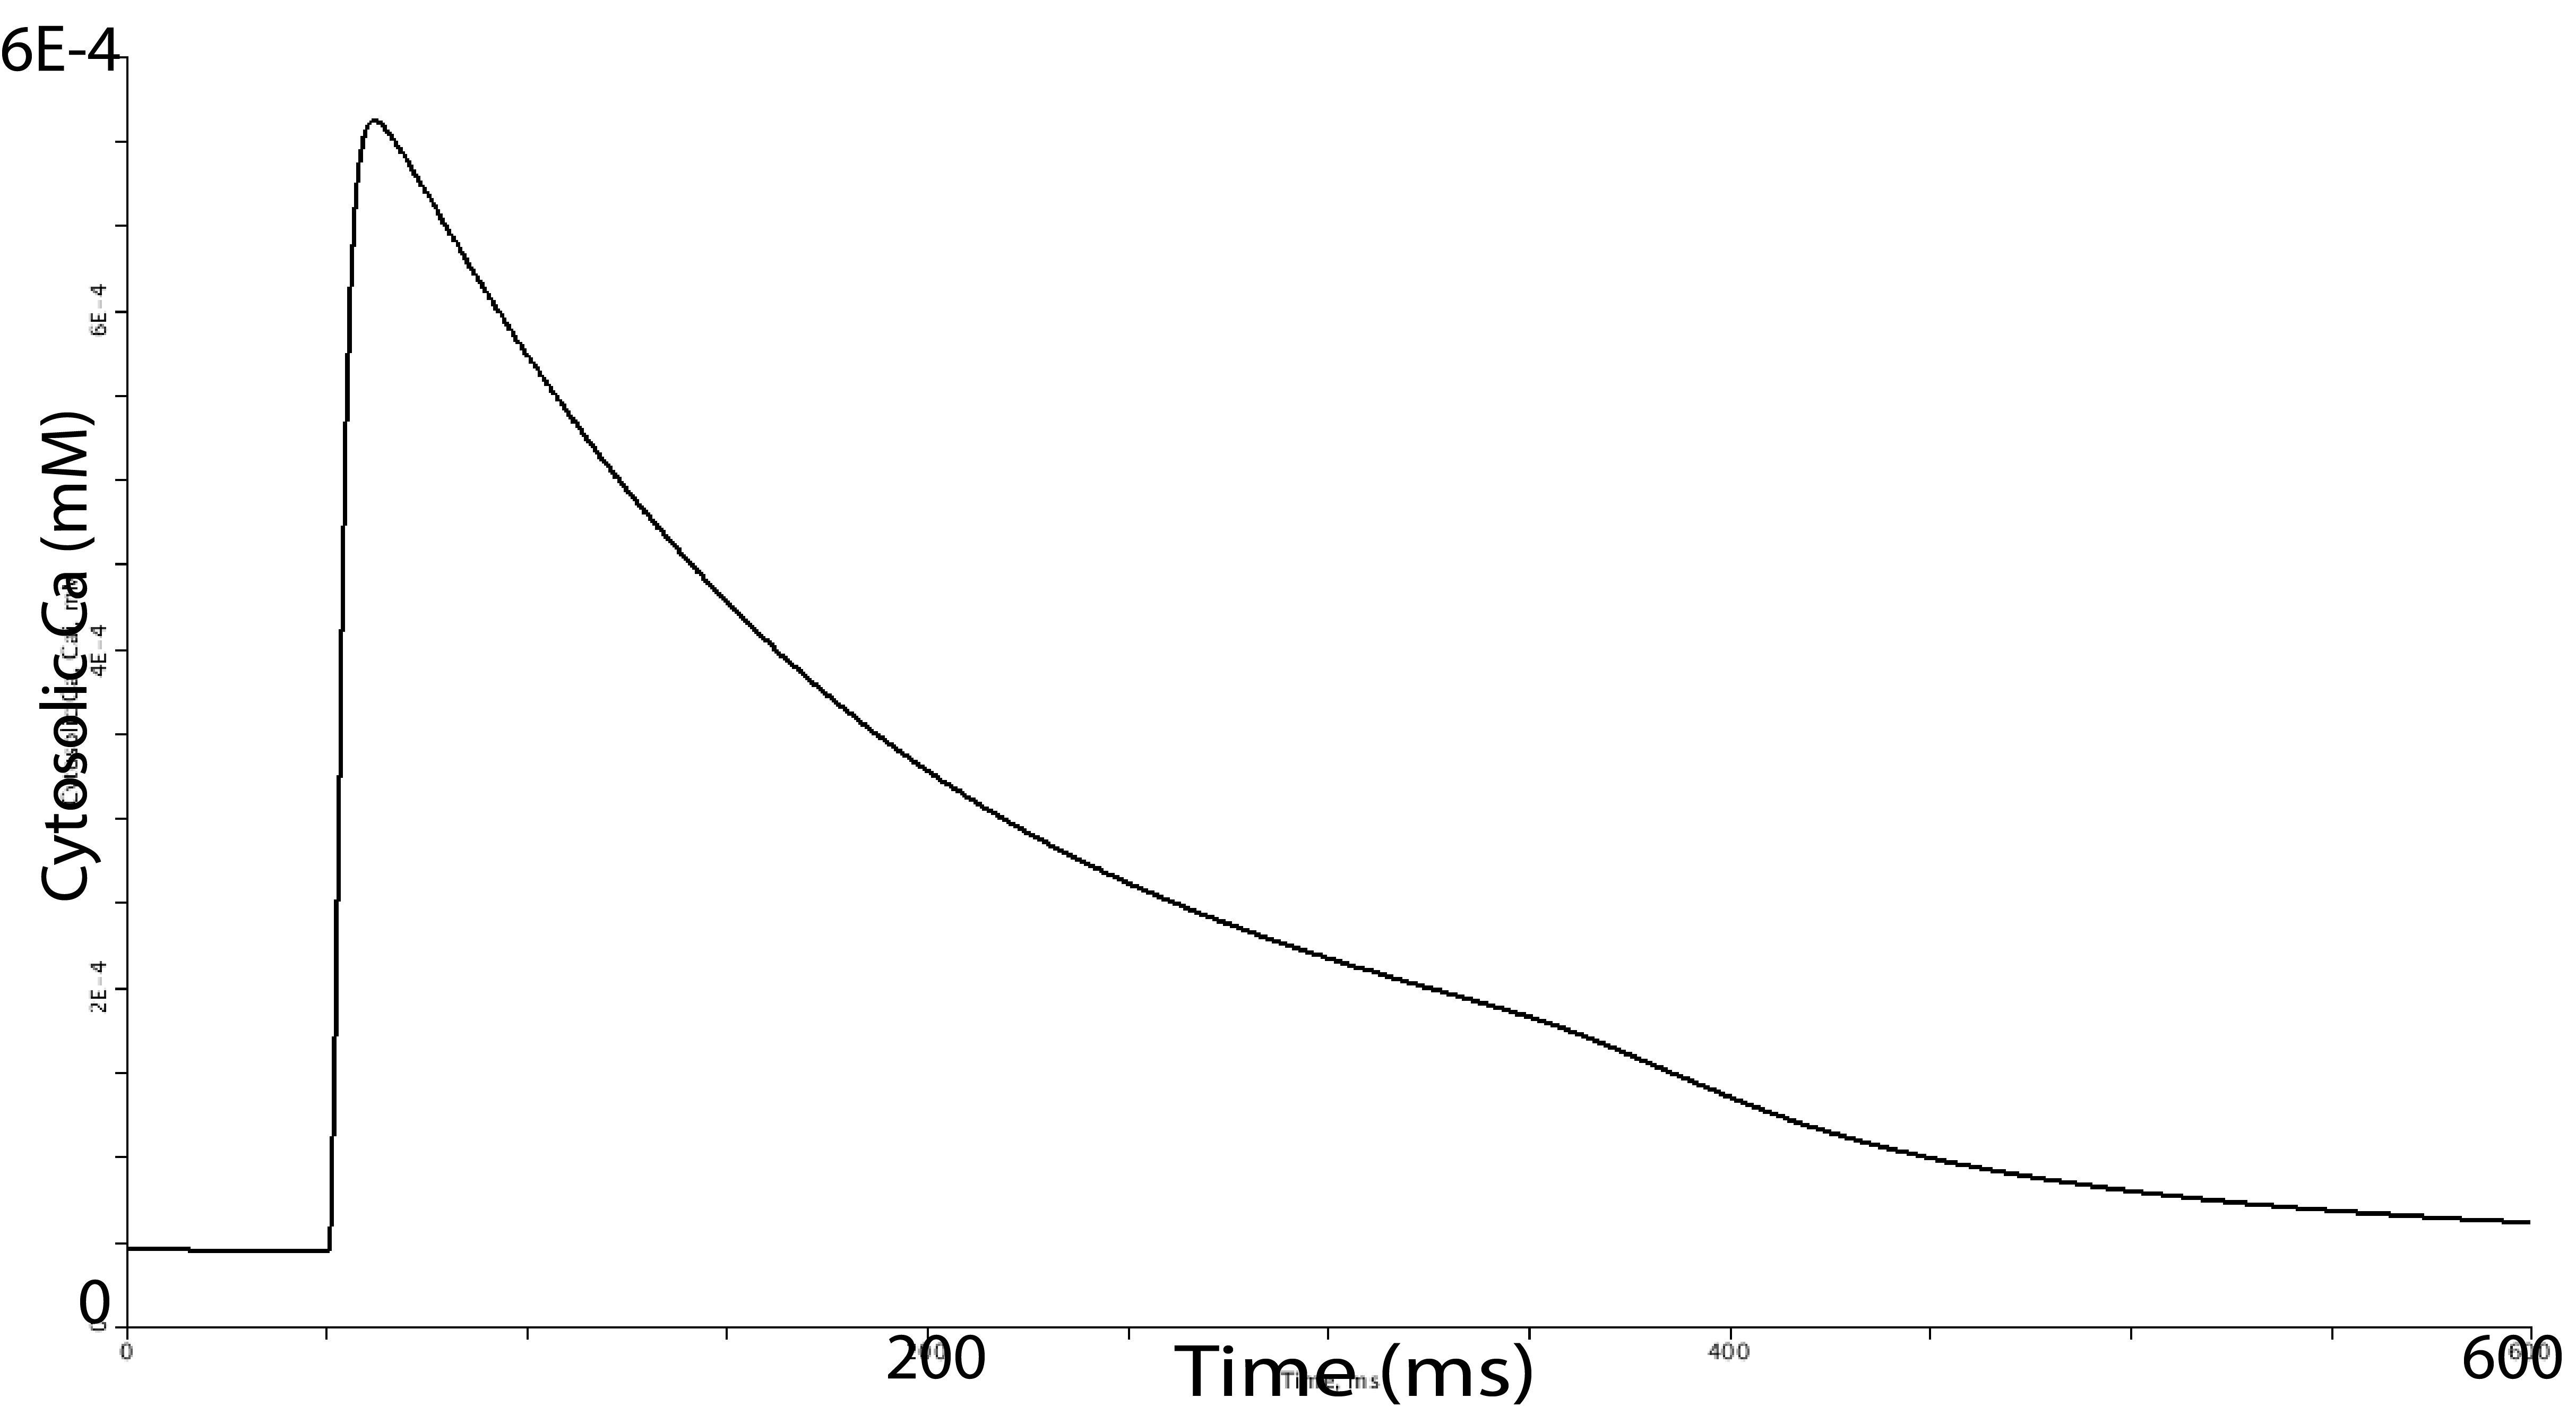
\includegraphics[width = \textwidth]{figs/200gcaledit.png}
		\caption{}
		\label{fig:right}
	\end{subfigure}
	\caption{Intracellular calcium concentration for each G\_Cal conductance. A: Conductance set to zero B. Conductance set to 50\% normal conductance, C: Conductance set to 100\% conductance, D: Conductance set to 200\% conductance. The time constant appears to be reduced with each conductance increase. Units on the graph are in concentration (millimolar) on the y axis and time (milliseconds) on the x axis}
	\label{fig:exp1}
\end{figure}

\rowcolors{2}{gray!25}{white}
\begin{table}[H]
	\centering
	\caption{Calculated APD90, Time to Peak (TTP), and Time constants for calcium transients resulting from the shown changes in the calcium channel conductance (g\_Cal)}
	\label{tab:calcium}
	\begin{tabular}{ccccc}
		\hline \hline
		Calcium Conductance & APD90  & Time To Peak  & Time Constant & R-squared\\ 
		L/(faradsSeconds) & (milliseconds) & (milliseconds)& (milliseconds)& \\
		\hline
		0\% Conductance & 74& 5.95&240 &0.858 \\ 
		50\% Conductance &222 &7.55 &204 &0.946 \\ 
		
		100\% Conductance & 278 &8.05 & 202& 0.977\\ 
		
		200\% Conductance& 344 & 8.70& 213& 0.995\\ 
		
		
		\hline 
		\hline
	\end{tabular} 
\end{table}

\begin{figure}[H]
	\centering
	\begin{subfigure}{0.45\textwidth}
		\centering
		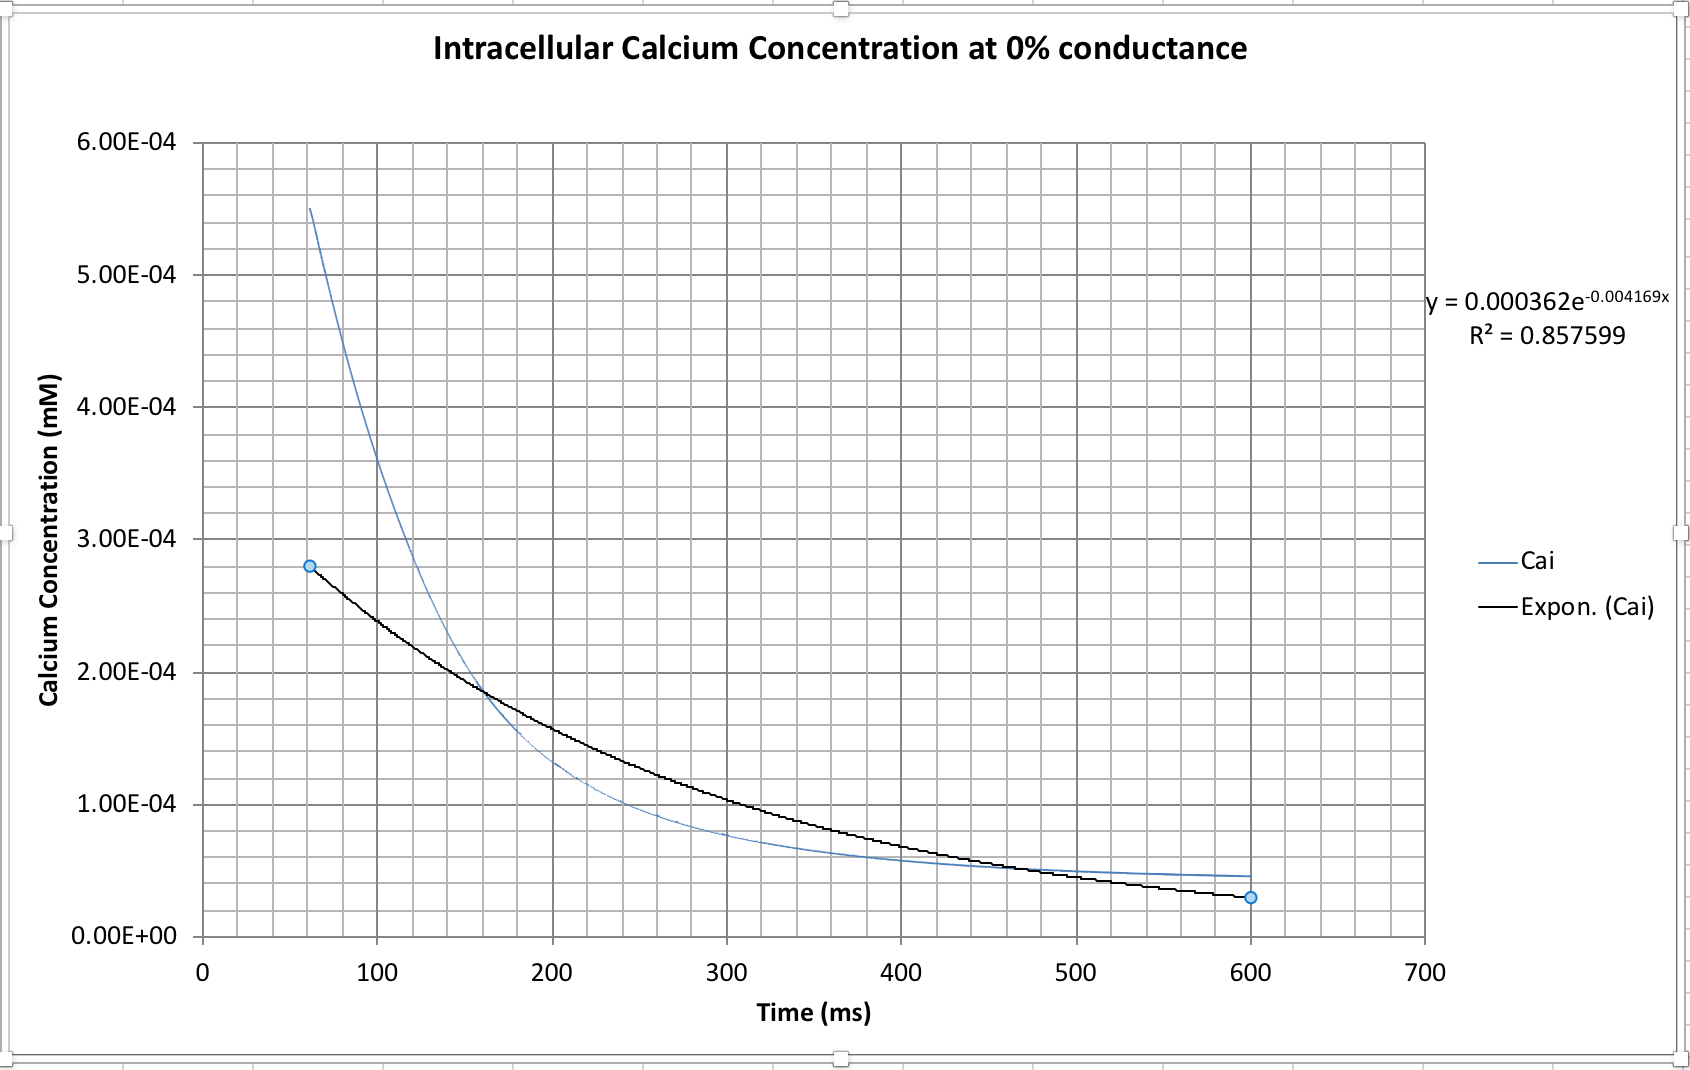
\includegraphics[width = \textwidth]{figs/3.png}
		\caption{}
		\label{fig:left}
	\end{subfigure}
	\begin{subfigure}{0.45\textwidth}
		\centering
		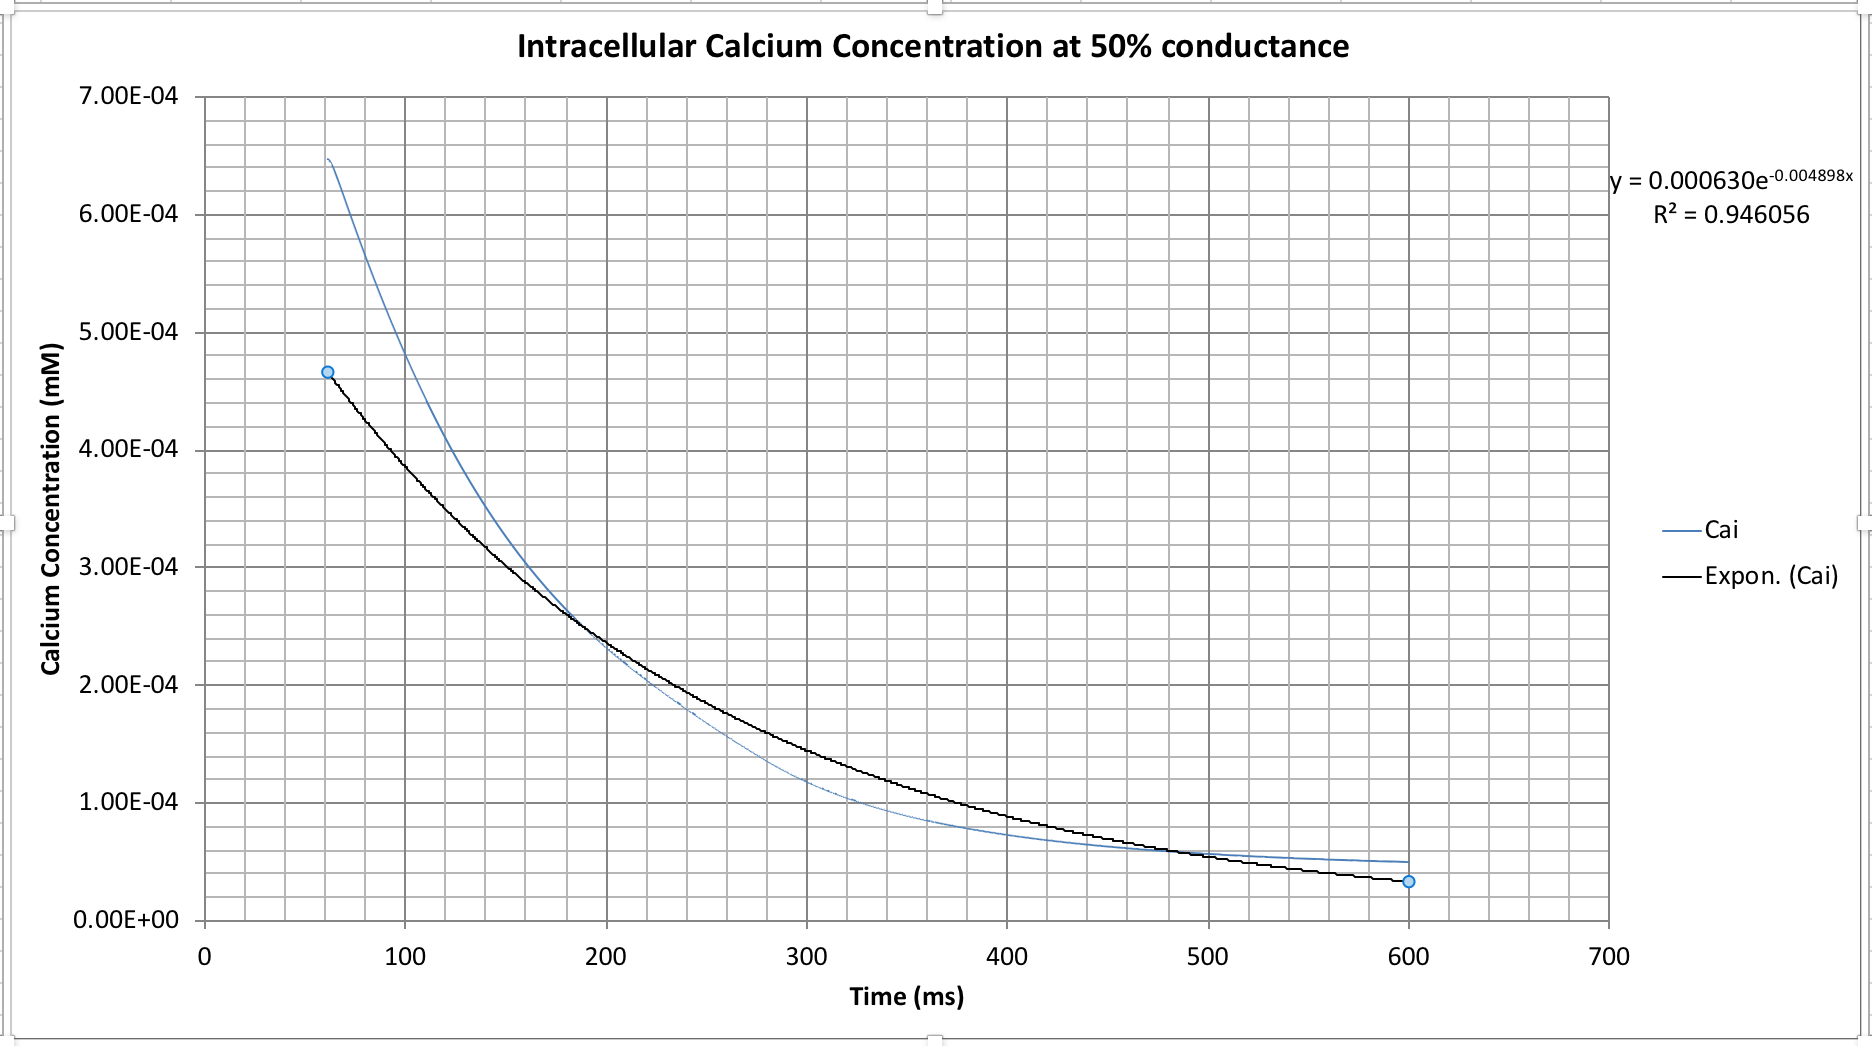
\includegraphics[width = \textwidth]{figs/2.png}
		\caption{}
		\label{fig:right}
	\end{subfigure}
	\vskip\baselineskip
	\begin{subfigure}{0.45\textwidth}
		\centering
		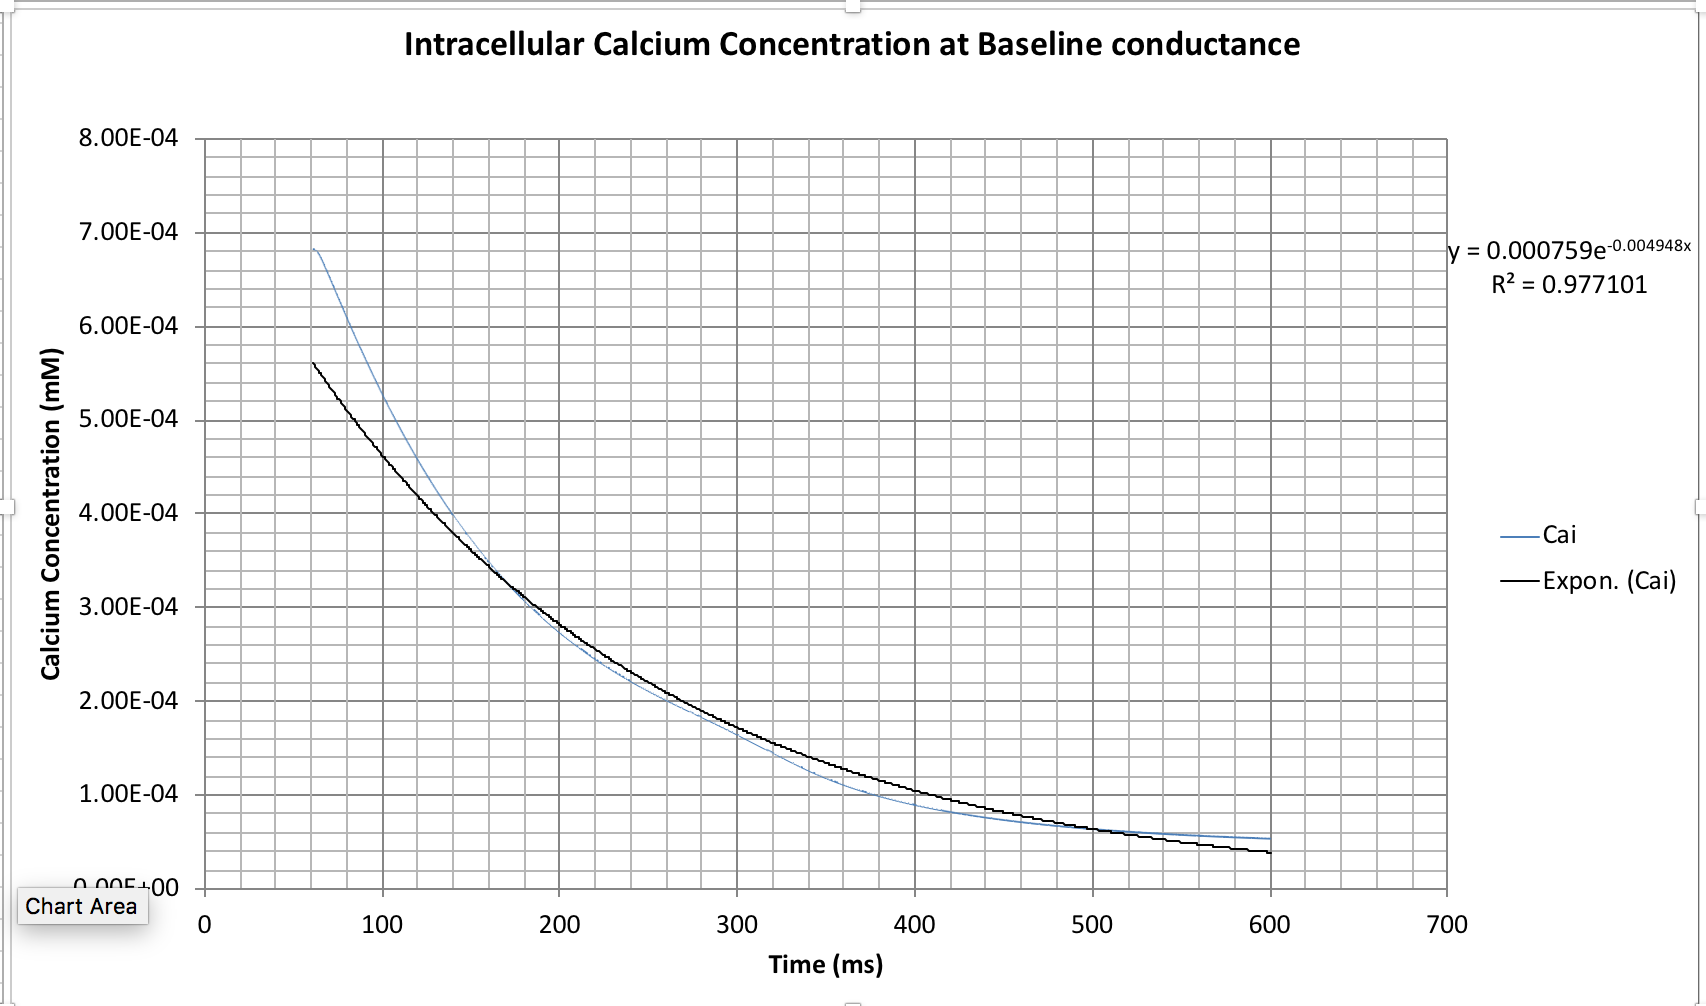
\includegraphics[width = \textwidth]{figs/1.png}
		\caption{}
		\label{fig:left}
	\end{subfigure}
	\begin{subfigure}{0.45\textwidth}
		\centering
		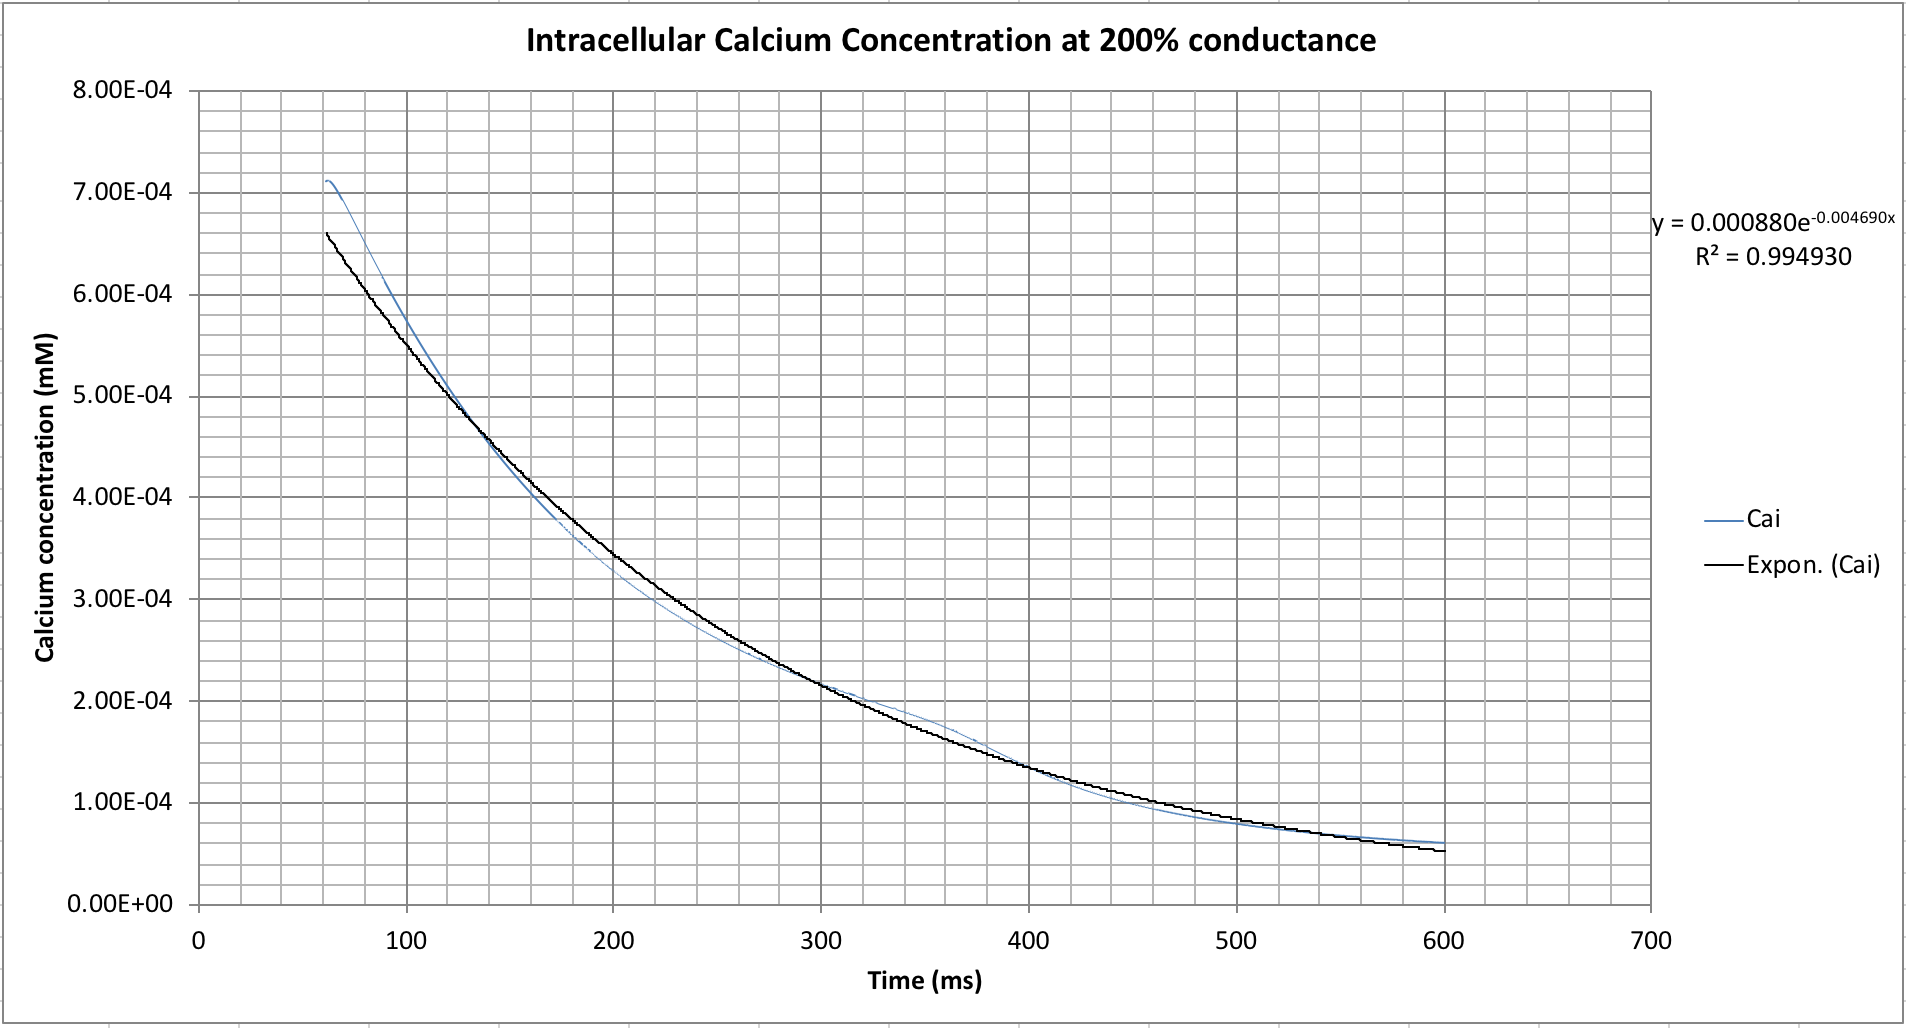
\includegraphics[width = \textwidth]{figs/4.png}
		\caption{}
		\label{fig:right}
	\end{subfigure}
	\caption{Summary figure of the intracellular calcium Decay with overlay concentration based on changes to the calcium conductance. A. Zero Conductance B. 50\% normal conductance, C. 100\% conductance, D. 200\% conductance. Units on the graph are in concentration (millimolar) on the y axis and time (milliseconds) on the x axis}
	\label{fig:overlays}
\end{figure}


\section{Conclusion}


\section{Appendix} 


%%%%%%%%%%%%%%%%%% Correct Bibliography Style

\bibliography{C:/Users/Jake/Documents/library}
\bibliographystyle{IEEEtran}


\end{document}


%%%%%%%%%%%%%%%% Table Example %%%%%%%%%%%%%%%%%%%%%%
\rowcolors{2}{gray!25}{white}
\begin{table}[H]
	\centering
	\caption{Simulated measurements for conduction velocity and maximal upstroke velocity}
	\label{tab:results}
\begin{tabular}{ccc}
	\hline \hline
	Experiment  & Conduction Velocity & Maximal Upstroke Velocity\\ 
	Number & (cm/ms)& (mV/ms) \\
	\hline
	 1 & 16.6389 &  69.8933 \\ 
	 2 &  18.9606&  73.9121 \\ 

	 3 &  24.7062&  83.871 \\ 

	  4&  45.2948&  109.1537\\ 

	  5&  52.6004&  116.8785\\ 

	  6&  77.6482&  131.6630\\ 

	  7&  2.0641&  0.0222\\ 

	  8&  44.0706&  109.3527\\ 

	  9&  45.2948&  109.1675\\ 

	  10&  2.1013&  -0.0024\\ 

	  11&  2.0896&  -0.0024\\ 

	  12&  60.3930&  179.3235\\ 
	  13&  38.8214&  86.8933 \\ 

	  14&  31.9728&  60.6956\\ 

	  15&  27.6375&  48.7076\\ 
	  16&  23.2945&  35.4873\\ 
	  17&  20.3827&  28.0958\\ 
	\hline 
	\hline
\end{tabular} 
\end{table}

%%%%%%%%%%%%%%%%% Figure Example %%%%%%%%%%%%%%%%%%%
	\begin{figure}[H]
	\centering
	\begin{subfigure}{0.49\textwidth}
		\centering
		\includegraphics[width = \textwidth]{../Simulation/Experiment_11.png}
		\caption{}
		\label{fig:left}
	\end{subfigure}
	\begin{subfigure}{0.49\textwidth}
		\centering
		\includegraphics[width = \textwidth]{../Simulation/Experiment_9.png}
		\caption{}
		\label{fig:right}
	\end{subfigure}
	\vskip\baselineskip
	\begin{subfigure}{0.49\textwidth}
		\centering
		\includegraphics[width = \textwidth]{../Simulation/Experiment_4.png}
		\caption{}
		\label{fig:left}
	\end{subfigure}
	\begin{subfigure}{0.49\textwidth}
		\centering
		\includegraphics[width = \textwidth]{stimulation.png}
		\caption{}
		\label{fig:right}
	\end{subfigure}
	\caption{Changes in Stimulation Current. (a) Output figure from experiment 11. (b) Output figure from experiment 9. (c) Output figure from experiment 4. (d) A summary figure showing the changes in conduction velocity and max dV/dt as the stimulation current varies. Note that once you exceed a certain threshold there is relatively no change to the conduction velocity or max dV/dt. }
	\label{fig:stimulation}
\end{figure}




